\documentclass[11pt]{article}

\usepackage[margin=1in]{geometry}
\usepackage[T1]{fontenc}
\usepackage{lmodern}
\usepackage{setspace}
\usepackage{amsmath}
\usepackage{tikz}
\usetikzlibrary{positioning}
\usepackage[table]{xcolor} % for \cellcolor and \rowcolor
\usepackage{amssymb}
\usepackage{array}
\usepackage{tabularx}
\usepackage{booktabs}

\newcommand{\panel}[1]{%
 \addlinespace[3pt]
 \rowcolor{gray!15}%
 \multicolumn{8}{@{}l}{\rule{0pt}{2.8ex}\textbf{\textsc{#1}}}\\
 \addlinespace[1pt]
}
\newcommand{\pbar}{\cellcolor{gray!35}{}} % panel bar cell
\newcommand{\nobar}{} % empty bar cell

\usepackage{amsthm}
\newtheorem{proposition}{Proposition}
\newtheorem{definition}{Definition}

\usepackage[round,authoryear]{natbib}
\setcitestyle{aysep={}}
\setcounter{secnumdepth}{0} % ARPE prints unnumbered headings
\usepackage{xurl}
\usepackage[colorlinks=true,
 linkcolor=black,
 citecolor=black,
 urlcolor=blue,
 pdftitle={Scarcity in an age of AI abundance},
 pdfauthor={Agisilaos Papadogiannis}]{hyperref}

\usepackage[labelfont=bf]{caption}
\doublespacing

\title{Scarcity in an age of AI abundance}
\author{Agisilaos Papadogiannis\thanks{Independent Researcher (PhD, MBA). Correspondence: \href{mailto:apapadogiannis@gmail.com}{apapadogiannis@gmail.com}. ORCID: \href{https://orcid.org/0009-0002-7753-7052}{0009-0002-7753-7052}.}}
\date{}

\begin{document}
\singlespacing
\hypersetup{urlcolor=black}
\maketitle

\begin{abstract}
A growing narrative in technology commentary and macroeconomics holds that advanced AI and robotics will deliver material abundance, near-zero marginal costs, and an end to economically meaningful scarcity. This paper challenges that view with two original concepts. \emph{AI technological abundance} (ATA) is a regime of strong cost compression and capability expansion in AI-intensive production, in which the marginal cost of many AI-mediated services falls sharply once systems are trained, deployed, and scaled. \emph{AI economic abundance} (AEA) is a strictly stronger outcome: broad affordability of an essential living-standards bundle, requiring that household resources keep pace with bundle prices. The central claim is that ATA does not in general deliver AEA. Cost compression does not eliminate scarcity; it reorganizes it, shifting binding constraints and migrating rents toward whatever remains scarce. We develop a five-layer framework in which scarcity and rent formation arise in (1) physical resources and space, (2) infrastructure such as energy, compute, and semiconductor fabrication, (3) capabilities and organizational know-how, (4) institutions that govern access and deployment, and (5) jurisdictions that supply enforcement and security. Ownership and control cut across all five layers, so who gains from AI depends jointly on where rents migrate and on each actor's claims across layers; AEA fails when rents rise in layers that weigh heavily in household budgets while household claims on those layers remain narrow. The framework is illustrated through the semiconductor supply chain and maps potential winners and losers, with implications for inequality, investment, and the political economy of transfers.
\end{abstract}

\noindent\textbf{Keywords:} Artificial intelligence, Scarcity, Inequality, Political economy, Infrastructure bottlenecks, Jurisdictional competition

\vspace{0.8em}
\noindent\rule{\textwidth}{0.4pt}

\vspace{0.4em}
{\small
\renewcommand{\arraystretch}{1.15}
\newcommand{\lnk}[2]{\href{#1}{\texttt{#2}}}
\noindent\begin{tabular}{@{}>{\raggedright\arraybackslash\bfseries}p{0.24\textwidth}>{\raggedright\arraybackslash}p{0.73\textwidth}@{}}
Forthcoming in &
\textit{Asian Review of Political Economy} (2027),\newline \lnk{https://doi.org/10.1007/s44216-026-00090-y}{doi.org/10.1007/s44216-026-00090-y}\newline
Please cite the published article.\\\noalign{\vskip 0.75em}
Code and data &
\lnk{https://github.com/apapadogiannis/ai-abundance}{github.com/apapadogiannis/ai-abundance}\newline
Archived at \lnk{https://doi.org/10.5281/zenodo.24441153}{doi.org/10.5281/zenodo.24441153}\newline
A record of the paper: its definitions, its model and its table as data. The paper is theoretical and has no computation to reproduce.\\\noalign{\vskip 0.75em}
Also by the author &
Other papers, code and tools: \lnk{https://github.com/apapadogiannis}{github.com/apapadogiannis}\\\noalign{\vskip 0.75em}
Notice &
\copyright\ 2026 The Author. Open access under the Creative Commons Attribution 4.0 International License. This file is the author's version of the accepted text.
\end{tabular}
}

\clearpage
\doublespacing
\hypersetup{urlcolor=blue}

%============================================================================
\section{Introduction}
\label{sec:intro}

Advanced AI and robotics are often discussed in the language of abundance and post-scarcity. This paper argues that the key issue is not whether AI can make many activities cheaper in principle, but where the binding constraints move as automation diffuses, and who controls the assets and rules that remain scarce.

Over the past decade, a specific narrative about advanced artificial intelligence (AI) and robotics has gained traction in technology writing, macroeconomic commentary, and popular books: powerful AI systems and widespread automation will not only raise productivity, but will eventually unwind scarcity itself. In its simplest form, the narrative runs in three steps: as AI systems and robots become more capable, and are assumed to improve or even self-improve with little friction, the marginal cost of producing many goods and services falls toward zero; competition and open access translate these cost reductions into falling prices and broad-based deflation, especially for digitally delivered or highly automated outputs; and, pushed far enough, the price system loses much of its informational and allocative role, so that society approaches a post-scarcity world in which work and capital ownership no longer matter in an economically meaningful way. This logic underpins influential books that anticipate near-zero marginal costs and a shrinking role for human labor and private ownership in economic life \citep{Rifkin2014, SrnicekWilliams2015, Bastani2019, Harari2016, Ford2015, Susskind2020, Moleka2025}.

To keep the discussion precise, we introduce two original concepts that the post-scarcity literature systematically conflates. \emph{AI technological abundance} (ATA) denotes a regime of strong cost compression and capability expansion in AI-intensive production, in which the marginal cost of many AI-mediated services falls sharply once systems are trained, deployed, and scaled. \emph{AI economic abundance} (AEA) denotes a strictly stronger, distributional and institutional outcome: broad affordability of an essential living-standards bundle, which requires that the gains from cost compression pass through to household living standards rather than being captured as rents by owners of scarce bottlenecks. Neither concept appears in the prior literature under these names or with this content; the ``A compact mathematical formulation'' section operationalizes AEA formally as a bundle-affordability condition.

The post-scarcity narrative presumes that ATA implies AEA. The central claim of this paper is that it generally does not. Even under ATA, \emph{binding constraints} (inputs or permissions that cannot scale without congestion, rationing, or rising shadow prices) can persist or tighten in complementary domains. The mechanism is straightforward. When AI makes some outputs cheaper to produce, the economy does not become unconstrained; it becomes constrained elsewhere. Lower effective costs expand scale and shift demand toward complementary inputs that are not freely replicable: energy and grid capacity, specialized compute hardware, data-center real estate, supply-chain resilience, trusted institutions, and regulatory permissions. These complements become bottlenecks; the rents they create accrue to whoever controls them, whether firms, platforms, or states; and whether households experience any meaningful form of AEA then depends on how those rents are competed away, regulated, taxed, or redistributed. Under ATA, scarcity therefore tends to migrate toward bottlenecks and control rights rather than disappearing.

Much of the techno-optimist narrative is framed as a progression from today's artificial narrow intelligence (ANI) to artificial general intelligence (AGI), artificial superintelligence (ASI), and finally a technological singularity in which machine intelligence rapidly outpaces human capabilities.\footnote{ANI: systems highly capable in specific tasks; AGI: hypothetical systems matching or exceeding human performance across most cognitive domains; ASI: systems vastly exceeding human capabilities in virtually all relevant tasks \citep{Bostrom2014}. The singularity is the conjectured point at which such systems drive runaway improvements in intelligence and growth \citep{Vinge1993}.} Classic treatments portray the singularity as a qualitative break in economic and social dynamics \citep{Kurzweil2005, Bostrom2014}, and recent contributions push the argument further: an ``intelligence inversion'' that turns cognition into an abundant commodity \citep{Mostaque2025}, an ``economic singularity'' driven by exponential technologies, cheap energy, and AI \citep{PalBittel2024}, scenarios in which AI systems design their own hardware and reshape economic and political structures \citep{Tegmark2017}, and trajectories of structural deflation and abundance extending to medicine and longevity \citep{DiamandisKotler2012, Booth2020, Diamandis2025LongevityGuidebook}. While the details differ, the shared mechanism is a strong form of cost compression: AI turns cognition and coordination into cheap inputs, competition passes the reductions through to prices, and the remaining bottlenecks are assumed small enough not to prevent broad affordability.

Taken literally, this is not a neutral extrapolation of current trends. It is a strong proposition about when technological abundance translates into economic abundance, and it requires six conditions to hold simultaneously: (i) AI systems can continue to improve and be deployed with few binding governance or safety constraints; (ii) energy and key natural resources become so abundant that they cease to be binding inputs; (iii) production capacity and supply chains can scale without persistent bottlenecks; (iv) goods, services, and ideas can be reallocated with negligible time delays or congestion; (v) geographic borders and jurisdictional boundaries do not materially restrict flows of data, capital, or AI services; and (vi) adoption is frictionless, meaning that organizations can integrate AI into real workflows without binding skill, trust, liability, or change-management constraints, and that key complements such as data rights, verification, and institutional legitimacy scale alongside deployment. These conditions are rarely made explicit in post-scarcity arguments, yet all six are needed for scarcity to disappear in the strong sense the rhetoric implies; once any one of them is relaxed, scarcity reappears somewhere in the system.

A large literature already treats AI as a powerful but essentially conventional technology: task-based models show how automation displaces some activities, complements others, and can widen inequality through the capital--labor split rather than through any collapse of economic constraints \citep[e.g.][]{AcemogluRestrepo2018,AcemogluRestrepo2021}, and the International Monetary Fund emphasizes that generative AI may boost output while increasing wealth inequality and cross-country divergence absent proactive policy \citep{IMF2024}. Neither this literature nor the post-scarcity narrative, however, provides a unified structural account of how scarcity migrates under large-scale AI deployment: the post-scarcity literature identifies the direction of change but does not model where binding constraints relocate or who captures the resulting rents, while the automation literature models distributional consequences without an economy-wide account of scarcity migration. This paper occupies the gap between them.

History offers a useful parallel. Mechanical refrigeration and refrigerated transport reduced the seasonality and local scarcity of perishables by integrating segmented markets and expanding effective supply. Yet scarcity did not vanish; it reappeared in the \emph{complements} required to realize the new abundance: refrigerated warehouses, specialized transport capacity, reliable energy, port-and-hub access, and the concentrated capital needed to build, coordinate, and govern the cold chain.\footnote{See \citet{GoodwinGrennesCraig2002} on refrigeration and market integration, and \citet{DelgadoPinillaAparicio2023} on refrigerated transport and international meat markets.} An innovation that compresses costs in one domain shifts binding constraints into infrastructure, institutions, and location, reallocating rents toward the owners and controllers of the new bottlenecks rather than eliminating rents altogether. AI-driven cost compression has the same structural implication: cheaper cognition does not remove constraints that are not cheaply replicable, and it can make the remaining constraints more binding: compute and cloud supply chains are concentrated, energy and grid access is increasingly salient for data centers, and policy discussions increasingly treat compute itself as a governance lever.

This paper takes an agnostic stance on whether AGI or ASI in the strongest sense is feasible. Rather than debating that frontier, it takes the optimists' premise seriously and asks a narrower question: even if very powerful AI and robotics are widely deployed, does scarcity disappear in any economically meaningful sense? The core move is to shift attention from the marginal cost of isolated goods to the economy-wide \emph{scarcity structure}: the configuration of binding constraints and rent formation in an AI-rich economy. The central claims are threefold:
\begin{enumerate}
 \item \textbf{ATA does not imply AEA.} Even dramatic cost compression in many goods and services, especially digital and cognition-intensive ones, need not translate into broad affordability of essential living conditions.
 \item \textbf{AI reorganizes scarcity.} Under ATA, binding constraints tend to shift rather than vanish. The paper models this as a reallocation of rents across five layers: (1) physical resources, energy, and space, (2) infrastructure (power grids, compute, fabs, data centers, automation), (3) capabilities and high-trust organizational know-how, (4) rules and institutions governing access, and (5) jurisdictions supplying enforcement capacity and security. Layers 4 and 5 are analytically distinct: institutions are the rule systems governing access and control; jurisdictions are the territorial entities that give those rules coercive force and enforce them at scale.
 \item \textbf{Distribution follows ownership.} Ownership and control cut across layers. The pattern of cross-layer claims held by firms, platforms, states, and households determines who captures the rents that persist under ATA, how gains split between capital and labor, and whether any meaningful degree of AEA emerges through wages, asset-linked claims, and transfers.
\end{enumerate}
In distributional terms, returns to both capital and labor increasingly depend on whether they are tied to \emph{post-AI bottlenecks} (layers where scarcity remains binding) rather than to domains where AI compresses costs and competition forces pass-through.

The remainder of the paper proceeds as follows. We first characterize ATA in operational terms and identify the domains in which cost compression is likely to be strongest, and then explain why entry into an ATA regime does not, in general, imply AEA. The paper next introduces the five-layer scarcity structure together with a minimal notation for layer rents and cross-layer exposure, describes how large-scale AI deployment reallocates scarcity across layers and maps schematic winners and losers, and finally turns to ownership and control, the state, comparative state-market configurations, and macro outcomes before concluding.

%==============
\section{Mechanisms and enablers of AI technological abundance}
\label{sec:abundance}

This section identifies the mechanisms that could generate ATA and clarifies where marginal costs can plausibly fall sharply. The discussion is intentionally schematic: AI can drive marginal costs toward very low levels for some digital outputs and selected routine physical services deployed at scale, while many physical, infrastructural, and institutional complements keep costs bounded away from zero elsewhere. The section surveys four domains of potential cost compression and two cross-cutting enablers that shape how these capabilities are deployed at scale (Figure~\ref{fig:abundance_domains_grid}).

\begin{figure}[t]
\centering
\begin{tikzpicture}[
 domainbox/.style={
 draw,
 rounded corners,
 minimum width=5.2cm,
 minimum height=2.0cm,
 align=center
 },
 overlay/.style={
 draw,
 rounded corners,
 thick
 },
 labelbox/.style={
 fill=white,
 inner sep=2pt,
 align=center
 }
]

% 2x2 domain boxes
\node[domainbox] (cog) at (-3.0, 1.4) {\textbf{Cognitive work}\\{\small Information services, coding, analysis}};
\node[domainbox] (phys) at ( 3.0, 1.4) {\textbf{Physical automation}\\{\small Robotics, logistics, manufacturing}};
\node[domainbox] (health) at (-3.0, -1.4) {\textbf{Health and medicine}\\{\small Diagnosis, discovery, care delivery}};
\node[domainbox] (sci) at ( 3.0, -1.4) {\textbf{Science and energy}\\{\small Materials, grids, resource frontiers}};

% Overlay rectangle for cross-cutting enablers
\draw[overlay] (-6.2,3.6) rectangle (6.2,-3.6);

% Overlay labels
\node[labelbox] at (0, 3.6) {\textbf{Agentic AI} (cross-cutting deployment mode)};
\node[labelbox] at (0,-3.6) {\textbf{Edge intelligence} (on-device compute substrate)};

\end{tikzpicture}
\caption{Mechanisms of AI technological abundance (ATA) across four domains. Agentic AI and edge intelligence are
cross-cutting enablers that scale coordination and execution and extend AI capability into devices and machines.
Unlike the four domains, which identify distinct sectors where cost compression occurs, the two enablers operate
across all domains simultaneously.}
\label{fig:abundance_domains_grid}
\end{figure}

%---------------------------------------------------------------------------
\subsection{Cognitive work and information services}

The first domain concerns cognitive and informational tasks. Large language models (LLMs) can already draft text, write and debug code, summarize documents, generate images and audio, and support decision-making at very low marginal cost once models are trained and deployed, which \citet{BrynjolfssonMcAfee2014} describe as a second machine age in which digital technologies increasingly automate cognitive work. Multimodal vision-language models extend these capabilities to images and video \citep{Jeong2024RobotLLM}, and tool-using LLMs can call external solvers, databases, and simulation engines, turning natural-language prompts into structured analytical pipelines \citep{Schick2023Toolformer}. In software engineering, code-generation assistants let developers specify high-level intent in natural language and delegate substantial blocks of implementation \citep{Ziegler2022NeuralCodeCompletion}. Because many digital outputs are non-rival, AI-based services can be replicated and distributed at very low marginal cost through cloud infrastructure. Cognitive work is therefore one of the primary domains in which ATA can plausibly arise.

%---------------------------------------------------------------------------
\subsection{Physical automation and service robotics}

The second domain is physical production and services. Industrial robotics, autonomous vehicles, and AI-guided machinery can reduce the cost of manufacturing, logistics, and a growing range of service tasks \citep{Ford2015, AcemogluRestrepo2018}. Beyond industrial settings, service robots are diffusing in transport and logistics, cleaning, hospitality, and selected care settings \citep{IFR2025ServiceRobotsBoom, Adeyemo2025UmbrellaRobotsNursing}, in bounded household tasks \citep{SahinGuvenc2007HouseholdRobotics}, in last-mile distribution \citep{DeMaioGhianiLaganaManni2024LastMile}, and in autonomous aerial systems for inspection, logistics, and defense \citep{Clapp2025MilitaryDronesEPRS}. A recent development is the rise of vision-language-action (VLA) models, which map visual observations and language goals directly into low-level robot actions, enabling general-purpose manipulation policies that transfer across tasks and embodiments \citep{Brohan2023RT2, Kawaharazuka2025VLA}; in the technological ideal, such systems turn robots into broadly capable workers that can be retasked by changing instructions rather than reprogramming control logic.

Embodied automation targets not only industrial output but also the marginal cost of routine service labor: cleaning, stocking, basic food preparation, simple inspection, warehouse picking, and other repetitive on-site workflows. In these cases, the economic margin is driven less by model inference cost than by capital amortization, utilization rates, maintenance, and safety assurance; the binding constraints shift from cognition to reliable embodiment, sensing, control, and liability in unstructured environments, a transition often described as a move from cognitive toward physical AI \citep{NvidiaPhysicalAI}. In the limiting case, basic goods could be produced at very low unit costs in highly automated facilities, subject to the energy, materials, and other complements analyzed in later sections.

%---------------------------------------------------------------------------
\subsection{\texorpdfstring{Health, medicine, and longevity}{Health, medicine, and longevity}}

The third domain concerns health and medicine. AI systems can already assist in image-based diagnosis, drug discovery, and the design of personalized treatment plans \citep{Topol2019}, and the success of AlphaFold in protein-structure prediction has strengthened the view that AI can accelerate biomedical research by large margins \citep{Jumper2021AlphaFold}. Public voices have pushed this logic further: Demis Hassabis has suggested that AI-driven scientific discovery could, within a decade, cure many or even all major diseases and contribute to ``radical abundance'' in health and energy \citep{Hassabis2025}. In the technological ideal, high-quality diagnostics and basic care can be delivered at very low marginal cost once models, clinical workflows, and delivery systems are scaled, though the extent to which this ideal can be realized depends on health-system capacity, regulation, liability and safety constraints, and other complements analyzed in later sections.

%---------------------------------------------------------------------------
\subsection{Scientific discovery, energy, and resource frontiers}

The fourth domain is the use of AI and robotics to accelerate scientific discovery and to transform energy and resource systems. Autonomous laboratories combine machine learning, robotics, and high-throughput experimentation to discover and synthesize new materials at scale \citep{Szymanski2023ALab}; DeepMind's GNoME system has identified hundreds of thousands of apparently stable new crystal structures with potential applications in batteries, photovoltaics, and other energy technologies \citep{DeepMindGNoME2023}. Related methods support battery informatics \citep{Ling2022BatteryInformatics}, plasma control in fusion research \citep{Degrave2022TokamakRL}, the optimization of power plants, grids, and renewables integration \citep{Entezari2023EnergyReview, IEA2023AI}, and AI-guided resource exploration. If AI and robotics compress the cost of scientific discovery and engineering design, the frontier of feasible technologies can move faster and open new energy and resource options: a form of technological abundance in innovation itself, whose realization and distribution nonetheless depend on the physical, infrastructural, and geopolitical constraints analyzed in later sections.

%---------------------------------------------------------------------------
\subsection{Cross-cutting enablers of ATA deployment}
\label{subsec:enablers}

The four domains above describe \emph{where} cost compression can occur. Two further elements shape \emph{how} these capabilities are deployed at scale. Unlike the four domains, which identify distinct sectors of activity, edge intelligence and agentic AI are enabling layers that operate across all four domains simultaneously, as Figure~\ref{fig:abundance_domains_grid} illustrates: edge intelligence provides the on-device compute substrate that extends AI into physical environments, and agentic AI provides the coordination and execution mode that scales AI activity within and across domains. Neither constitutes a separate source of cost compression in its own right; both amplify and condition the domain-level mechanisms.

\subsubsection{Edge intelligence (on-device compute substrate)}\label{subsec:edge}

Edge AI runs models close to the data source, on phones, vehicles, robots, sensors, and industrial controllers, reducing latency, improving reliability under connectivity constraints, and mitigating privacy and data-governance frictions because sensitive inputs need not leave the local environment \citep{Singh2023EdgeAI}. As specialized neural accelerators diffuse into consumer and industrial hardware, a growing share of inference cost is paid upfront as device capital expenditure rather than as metered cloud usage. This expands the set of economically viable AI services in the physical world and supports deployments ranging from microcontroller-class devices to on-device foundation models. Marginal costs can fall sharply for many perception, prediction, and control tasks, even though total system costs remain bounded by hardware, power, and deployment constraints.

\subsubsection{Agentic AI (cross-cutting deployment mode)}\label{subsec:agentic}

Agentic AI systems are software agents that do not simply answer prompts but pursue goals over time, call tools and external services, interact with platforms, and coordinate with other agents under limited human supervision \citep{Xi2025LLMAgents}; embodied through VLA models, they can sense, reason, and act in the physical world \citep{Kawaharazuka2025VLA}. Agentic AI has two distinct effects for ATA. First, it reduces the effective cost of coordination and management tasks that previously required human attention: scheduling, procurement, and routine back-office functions can in principle be executed by fleets of agents operating continuously. Second, it increases the scalability of both firms and individuals, since a small management team can supervise a much larger set of parallel activities when most steps are carried out by agents \citep{HadfieldKoh2025Agents, TanHuang2025AgentEconomy}; industry analyses anticipate an ``agentic commerce'' economy in which consumer-facing agents shop, negotiate, and transact on behalf of households and firms \citep{McKinsey2025AgenticCommerce, Citi2025AgenticAI}. In practice, deployment is mediated by access to models, compute, data, and platforms, and by concerns about trust, alignment, and control \citep{Sastry2024ComputeGovernance, Papagiannidis2025ResponsibleAIGovernance, Ngo2024AlignmentDeepLearning}. Agentic AI is thus a powerful amplifier of cost compression, but it also clarifies why capability does not automatically translate into broad-based abundance: agents scale execution while intensifying competition for the complements they require: compute, energy, privileged data, platform access, regulatory permissions, and trusted control interfaces.

%%%%%%%%%%%%%%%%%%%%%%%%%%%%%%%%%%%%%%%%%%%%%%%%%%%%%%%%%%%%%%%%%%%%%%%%%
\section{From cost compression to living standards}
\label{sec:ata_not_aea}

Across cognitive work, physical automation, health, and scientific discovery, AI systems act as cost compressors: they lower the marginal cost of many tasks and services and expand the feasible set of goods, experiences, and technologies the economy can provide. This section explains why that is not sufficient for abundance in living standards.

\paragraph{Point A (entry into ATA).}
We refer to \emph{Point A} as the regime boundary at which these mechanisms become scalable and persistent rather than episodic. Past Point A, a large and economically meaningful set of AI-intensive services can be supplied at very low marginal cost, so that cost compression becomes a structural feature of production in those domains. Point A is not a single milestone such as AGI; it is a deployment threshold at which models, tools, and robotic systems become reliable enough and cheap enough that many tasks can be executed at scale, and the binding constraints begin to shift away from cognition toward the complements required to deliver services in the real economy.

Figure~\ref{fig:ata_aea_quadrants} summarizes the distinction at the center of the paper. Crossing Point A moves the economy into an ATA regime. That transition does not, by itself, determine whether households experience a broad erosion of economically relevant scarcity in material living conditions, which we call AEA. ATA is a property of production possibilities in some domains; AEA is an outcome of pass-through, bottlenecks, and distribution.

\begin{figure}[t]
\centering
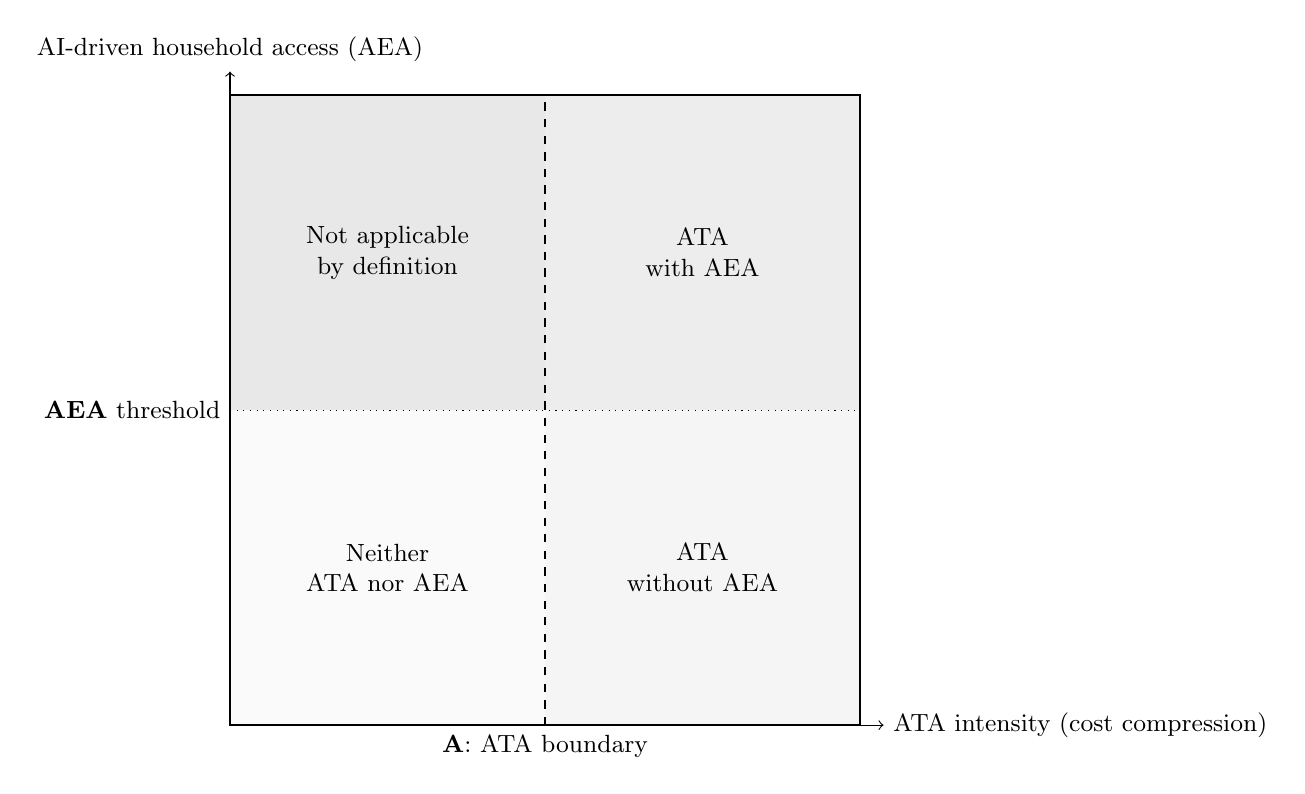
\begin{tikzpicture}[
 font=\small,
 q/.style={align=center},
 box/.style={draw, line width=0.6pt},
 shadeA/.style={fill=gray!8},
 shadeB/.style={fill=gray!14},
 shadeC/.style={fill=gray!4},
 shadeNA/.style={fill=gray!18}
]
 % Axes limits (chosen for equal quadrants)
 \def\xmax{8}
 \def\ymax{8}
 \def\xcut{4} % ATA boundary (midpoint)
 \def\ycut{4} % AEA threshold (midpoint)

 % Midpoints for labels (compute once)
 \pgfmathsetmacro{\xmidL}{\xcut/2}
 \pgfmathsetmacro{\xmidR}{(\xcut+\xmax)/2}
 \pgfmathsetmacro{\ymidB}{\ycut/2}
 \pgfmathsetmacro{\ymidT}{(\ycut+\ymax)/2}

 % Shaded quadrants
 \path[shadeC] (0,0) rectangle (\xcut,\ycut);
 \path[shadeA] (\xcut,0) rectangle (\xmax,\ycut);
 \path[shadeNA] (0,\ycut) rectangle (\xcut,\ymax);
 \path[shadeB] (\xcut,\ycut) rectangle (\xmax,\ymax);

 % Outer border
 \draw[box] (0,0) rectangle (\xmax,\ymax);

 % Axes
 \draw[->] (0,0) -- (\xmax+0.3,0) node[right]{ATA intensity (cost compression)};
 \draw[->] (0,0) -- (0,\ymax+0.3) node[above]{AI-driven household access (AEA)};

 % Regime boundaries
 \draw[dashed] (\xcut,0) -- (\xcut,\ymax);
 \node[below] at (\xcut,0) {\textbf{A}: ATA boundary};

 \draw[dotted] (0,\ycut) -- (\xmax,\ycut);
 \node[left] at (0,\ycut) {\textbf{AEA} threshold};

 % Quadrant labels
 \node[q] at (\xmidL,\ymidB) {Neither\\ATA nor AEA};
 \node[q] at (\xmidR,\ymidB) {ATA\\without AEA};
 \node[q] at (\xmidL,\ymidT) {Not applicable\\by definition};
 \node[q] at (\xmidR,\ymidT) {ATA\\with AEA};

\end{tikzpicture}
\caption{Four conceptual states. Entering ATA (to the right of Point A) does not guarantee AI-driven household abundance (AEA). The top-left quadrant is ruled out if AEA is defined as an AI-driven outcome.}
\label{fig:ata_aea_quadrants}
\end{figure}

Post-scarcity narratives typically treat the transition past Point A as sufficient for AEA. For that inference to hold, cost compression must pass through into lower effective household prices and must not be offset by constraints that become more salient as AI diffuses; those steps are mediated by market structure, institutions, and political economy. Four mechanisms can break the implied link.

\paragraph{Market structure and pass-through.}
Cost reductions do not automatically become lower household prices. When firms control critical platforms, infrastructures, or supply chains, a large share of the surplus created by ATA can be retained as profits or rents rather than passed through to consumers \citep{OECD2025AIInfra}.

\paragraph{Shifting bottlenecks and complementary scarcities.}
Even if many downstream AI-enabled services become cheap, tight constraints can persist or intensify in complements such as energy and grid access, compute capacity and semiconductor supply, high-quality data and rights of use, regulatory permissions, and trust and verification \citep{OECD2025AIInfra, Sastry2024ComputeGovernance, IEA2025EnergyAI}. In that case, some prices fall while others rise, and scarcity remains economically meaningful because the household budget constraint is tightened by what remains scarce, not by what becomes cheap.

\paragraph{Distribution and ownership.}
Even when aggregate productivity rises, household access can improve only weakly if the assets that capture the remaining rents are narrowly owned. The gains from cost compression then accrue primarily to capital owners, and living standards depend on whether and how those gains are shared through wages, competition, or transfers \citep{IMF2024}. These mechanisms also operate through labor markets: automation and task recomposition imply that some occupations contract while others expand, with distributional consequences that depend on how gains are shared between capital and labor \citep{IMF2024}.

\paragraph{The digital access threshold.}
Cost compression under ATA is conditional on digital access. Households without reliable connectivity, devices, or digital literacy cannot benefit from falling marginal costs in AI-mediated services regardless of how low those costs fall. According to data from China's internet regulator, roughly one-fifth of China's population remains outside the digital economy \citep{CNNIC2024}, and the International Telecommunication Union reports that approximately 2.6 billion people globally remain offline \citep{ITU2023}. For these populations, ATA generates no pass-through benefit whatsoever: they sit outside the perimeter within which cost compression operates. In the formal terms introduced below, the household claims \(\omega_{h\ell}\) are effectively zero across multiple layers simultaneously, not because rents are concentrated, but because the household is not connected to the system that generates them at all. Closing this access gap itself requires capital-intensive infrastructural investment (Layer 2), governed by institutional rules and access rights (Layer 4) and delivered through jurisdictional state capacity (Layer 5), investments that tend, absent deliberate public provision, to replicate the same bottleneck ownership patterns the framework identifies elsewhere \citep{ITU2023, IMF2024}.

ATA is thus neither sufficient nor necessary for AEA: cost compression can coexist with heightened scarcity in access and opportunity when bottlenecks and ownership concentrate the gains, while living standards can improve through institutional reform and redistribution even without frontier AI. The remainder of the paper makes this argument explicit through a five-layer scarcity structure that applies both before and after ATA: Point A shifts which layers bind most tightly, and ownership determines whether the surplus is transmitted to households.

%%%%%%%%%%%%%%%%%%%%%%%%%%%%%%%%%%%%%%%%%%%%%%%%
\section{The structure of scarcity}
\label{sec:framework}

The preceding section argued that entering an ATA regime does not by itself deliver AEA. The reason is structural: even if AI compresses marginal costs in many tasks and services, economies remain organized around the constraints that continue to bind, and around who controls the assets and rules that govern those constraints. This section introduces a scarcity-structure framework that makes that logic explicit, shifting the analysis from the marginal cost of particular outputs to an economy-wide map of where scarcity can bind and how ownership transmits rents across domains.

\begin{figure}[t]
\centering
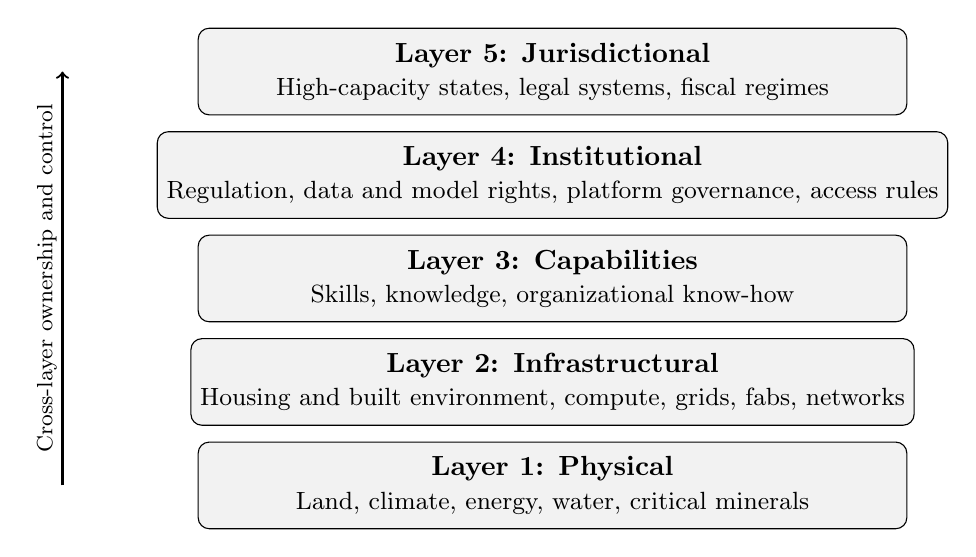
\begin{tikzpicture}[
 layerbox/.style={
 draw,
 rounded corners,
 minimum width=9cm,
 minimum height=1.1cm,
 align=center
 },
 node distance=0cm
]

% Layers (top to bottom)
\node[layerbox, fill=gray!10] (jur) {\textbf{Layer 5: Jurisdictional} \\ \small High-capacity states, legal systems, fiscal regimes};
\node[layerbox, fill=gray!10, below=0.2cm of jur] (inst) {\textbf{Layer 4: Institutional} \\ \small Regulation, data and model rights, platform governance, access rules};
\node[layerbox, fill=gray!10, below=0.2cm of inst] (cap) {\textbf{Layer 3: Capabilities} \\ \small Skills, knowledge, organizational know-how};
\node[layerbox, fill=gray!10, below=0.2cm of cap] (inf) {\textbf{Layer 2: Infrastructural} \\ \small Housing and built environment, compute, grids, fabs, networks};
\node[layerbox, fill=gray!10, below=0.2cm of inf] (phys) {\textbf{Layer 1: Physical} \\ \small Land, climate, energy, water, critical minerals};

% Ownership arrow on the left
\node[left=1.5cm of inf] (ownstart) {};
\draw[->, thick] (phys.west -| ownstart) -- (jur.west -| ownstart)
 node[midway, xshift=-0.2cm, rotate=90, anchor=center] {\footnotesize Cross-layer ownership and control};

\end{tikzpicture}
\caption{Five layers of scarcity and a cross-layer channel of ownership and control. The layers are present
in any complex economy. Under ATA, the tightness of constraints shifts across layers and the distributional
outcomes depend on who controls the assets and bottlenecks within and across layers.}
\label{fig:ai_scarcity_stack}
\end{figure}

\subsection{From asset-level scarcity to economy-wide constraints}

Earlier work models economic scarcity as an intrinsic, asset-level property that arises from the interaction of constrained supply and demand-side desirability \citep{PapadogiannisScarcity2025}: scarcity is treated as a latent, time-varying state variable shaped by economic pressures on demand and supply, and monetization functions map scarcity states into cash flows, so that discounted cash flow logic prices intertemporal scarcity across asset classes. This micro-level concept is useful for valuation because it links scarcity directly to prices and expected returns for a specific asset. On its own, however, it does not describe how scarcity is distributed across the economic system or how that distribution changes when a general-purpose technology such as advanced AI arrives. For that, we need a structural perspective in which scarcity is an economy-wide configuration of binding constraints rather than a property of individual assets.

\subsection{Five layers of economic scarcity}
\label{subsec:five_layers}

We define the \emph{scarcity structure} of an economy as the configuration of binding constraints that shape production, allocation, and distribution at a given point in time. These constraints are not limited to physical resources: they include infrastructural bottlenecks, limits in human and organizational capabilities, institutional restrictions, and the jurisdictional environment in which firms and households operate. Scarcity, in this sense, is not a single scalar but a multi-dimensional pattern. A key assumption in what follows is that the same structural layers exist both before and after the onset of ATA. What changes with ATA is not the taxonomy of scarcity but the tightness and interaction of constraints across layers: advanced AI can relax some margins of scarcity while simultaneously tightening others, especially by increasing demand for scarce complements.

The choice of five layers rather than a smaller set reflects specific analytical requirements. Three-tier frameworks organized around cross-cutting properties such as ownership, access, and control are useful for describing how rents are captured, but they conflate the structural sources of scarcity with the mechanisms of distribution. The five-layer structure keeps these separate: layers 1 through 5 identify where binding constraints arise, while the ownership matrix $O$ and cross-layer exposure profiles describe who captures the resulting rents. This separation is what makes the formal statement in the next section and Table~\ref{tab:rent_shift_layers} analytically tractable. Collapsing layers would prevent the framework from distinguishing, for example, between the institutional rules governing chip access and the jurisdictional enforcement capacity that makes those rules credible, a distinction the semiconductor illustration below shows to be economically consequential.

This paper therefore proposes a five-layer representation of the scarcity structure:

\begin{enumerate}
 \item \textbf{Physical layer}: the underlying material endowments of the economy, such as land and location, climate, water, energy resources, and critical minerals. These determine what can be produced in principle and how exposed an economy is to ecological limits and climate risk \citep[e.g.][]{Rockstrom2009}.

 \item \textbf{Infrastructural layer}: the capital-intensive systems that transform, store, and move physical resources and deliver essential services, including the built environment and housing stock, compute capacity and data centers, advanced semiconductor fabrication, automated production lines, power plants and grids, and transport, logistics, and communication networks. These infrastructures often exhibit scale economies, network effects, and long build times, which makes them natural bottlenecks \citep{OECD2024AIData,OECD2025AIInfra}.

 \item \textbf{Capabilities layer}: embodied and organizational knowledge, covering worker skills and human capital, tacit know-how, scientific and engineering expertise, and the routines and management practices through which firms turn infrastructures into effective production \citep[e.g.][]{Becker1993HumanCapital,NelsonWinter1982,Teece1997DynamicCapabilities}, as well as intangible capital such as reputations and brands. This is the layer where competition for frontier talent lives most directly, and where ATA automates many tasks while potentially raising the premium on a narrower set of complementary skills.

 \item \textbf{Institutional layer}: the formal and informal rules that govern access to and use of resources, infrastructures, and capabilities: zoning and permitting, grid interconnection rules, safety and liability regimes, intellectual property and data rights, competition policy and platform governance, and licensing and export controls. Scarcity here arises from regulatory and contractual barriers to entry and from the way rules allocate control and residual claims \citep[see][]{North1990Institutions, AcemogluRobinson2012}.

 \item \textbf{Jurisdictional layer}: access to high-capacity, high-trust states that can credibly enforce property rights and contracts, provide predictable regulation and taxation, and sustain stable monetary and fiscal regimes. Because state capacity, geopolitical position, and institutional quality differ across countries, scarcity appears as rationed access to residency and citizenship, secure legal protection, reliable financial rails, and market access under trusted courts and regulators \citep[e.g.][]{BesleyPersson2009StateCapacity}.
\end{enumerate}

The institutional and jurisdictional layers are closely related but analytically distinct. The institutional layer refers to rule systems and governance arrangements that shape access and control; these can operate inside firms, across platforms, or through international regimes independently of any particular territory. The jurisdictional layer captures the bundling of rules with territorial sovereignty, physical enforcement capacity, and geopolitical position. Two states may adopt formally similar institutions yet differ sharply in jurisdictional scarcity because only one can credibly enforce contracts at scale, backstop key infrastructures, or provide the security guarantees that attract mobile capital and talent. In short, institutions are the rules; jurisdictions are the territorial entities that give those rules coercive force and geopolitical weight. Institutional rents arise from who controls access under a given rule system, while jurisdictional rents arise from which territory can credibly supply and enforce those rules. Positional goods such as status, attention, and access to elite networks remain scarce even in very rich societies \citep{Hirsch1995}; in this framework they are treated as endogenous outcomes of interactions across layers rather than as a separate layer.

The layers in Figure~\ref{fig:ai_scarcity_stack} form a vertical stack but not a ranking. Physical endowments support infrastructures, which are operated through capabilities, governed by institutions, and bundled within jurisdictions; at any given time, any layer can be the binding constraint. The scarcity structure is the pattern of binding constraints across layers and their interactions: infrastructural scarcity in compute and power can amplify institutional scarcity in access to leading models, and jurisdictional scarcity in high-capacity states can amplify capabilities scarcity by concentrating firms, talent, and capital in a small set of places.

%%%%%%%%%%%%%%%%%%%%%%%%%%%%%%%%%%%%%%%%%%%%%%%%%%%%%%%%%%%%%%%%%%%%%%
\section{A compact mathematical formulation}
\label{sec:formal}

This section provides the minimal notation that the argument requires; the paper's case is deductive, and it does not depend on the formalism. The notation serves one essential purpose: it allows the central claim, that ATA does not imply AEA, to be stated as a falsifiable condition (Proposition~\ref{prop:not_sufficient}) that identifies precisely which parameters determine whether cost compression reaches households. Readers primarily interested in the qualitative argument may treat the proposition as a precise restatement of the verbal claim.

Index the five scarcity layers by \(\mathcal{L}=\{1,\dots,5\}\), corresponding to the physical, infrastructural, capabilities, institutional, and jurisdictional layers introduced above, and let
\begin{equation}
R_t=(R_{1,t},R_{2,t},R_{3,t},R_{4,t},R_{5,t})
\label{eq:rent_vector}
\end{equation}
denote the layer-level rent vector at date \(t\), where \(R_{\ell,t}\ge 0\) is total rent attributable to bottlenecks in layer \(\ell\), summed across all actors; \(R_{\ell,t}\) is higher when scarcity in layer \(\ell\) binds more tightly.

To incorporate ownership, index actors (or representative groups) by \(i=1,\dots,N\); actors may be firms, platforms, states, institutional investors, or households. Define an \emph{ownership matrix}
\begin{equation}
O=(O_{i\ell})_{i=1,\dots,N;\;\ell\in\mathcal{L}},
\qquad
\sum_{i=1}^N O_{i\ell}=1 \ \text{ for each } \ell\in\mathcal{L},
\label{eq:ownership_matrix}
\end{equation}
where \(O_{i\ell}\in[0,1]\) measures actor \(i\)'s share of effective control or residual claims over rents generated in layer \(\ell\). Assuming layer rents are allocated proportionally to ownership shares, the total rent income of actor \(i\) at date \(t\) is
\begin{equation}
\Pi_{i,t}=\sum_{\ell\in\mathcal{L}} O_{i\ell}\,R_{\ell,t},
\label{eq:rent_income}
\end{equation}
so distributional outcomes depend jointly on the time-varying rent vector \(R_t\) and the cross-layer ownership profile \(O\). Represent ATA by a regime parameter \(a\) that shifts the level and composition of the rent vector, \(R_{\ell,t}=R_{\ell,t}(a)\): moving from \(a=a^-\) to \(a=a^+\) can reduce some components and increase others. A strict post-scarcity limit corresponds to \(R_{\ell,t}=0\) for all \(\ell\), in which case \eqref{eq:rent_income} implies \(\Pi_{i,t}=0\) for all actors; this benchmark clarifies what strong post-scarcity rhetoric would require. The economically relevant question is instead how ATA changes the \emph{composition} of \(R_t\) and how those changes interact with \(O\).

To state what it means for cost compression to translate into broad economic abundance, fix a reference bundle \(b\) representing a minimum standard of living (energy services, shelter, basic health care, basic mobility, connectivity), and let \(P_t(b)\) denote the minimum expenditure needed to obtain \(b\) at date \(t\). Households \(h\in\mathcal{H}\) have disposable resources
\begin{equation}
Y_{h,t}:=W_{h,t}+\sum_{\ell\in\mathcal{L}} \omega_{h\ell}\,R_{\ell,t}+T_{h,t},
\label{eq:household_resources}
\end{equation}
where \(W_{h,t}\) is labor income, \(T_{h,t}\) net transfers, and \(\omega_{h\ell}\in[0,1]\) the household's effective claim on layer-\(\ell\) rents (directly or through asset ownership and intermediaries).

\begin{definition}[AEA: bundle-affordability condition]
\label{def:aea_formal}
AEA holds at date \(t\) if every household can afford the reference bundle \(b\), that is, \(Y_{h,t}\ge P_t(b)\) for all \(h\in\mathcal{H}\).
\end{definition}

To connect the scarcity structure to the cost of the bundle, define the \emph{price-relevant rent intensity} \(r_{\ell,t}:=\nu_{\ell,t}R_{\ell,t}\), where \(\nu_{\ell,t}\ge 0\) maps total rents into a comparable intensity (for example, rent per unit of bundle-relevant usage), and write the bundle price as
\begin{equation}
P_t(b)=\bar{C}_t(b)+\sum_{\ell\in\mathcal{L}} \kappa_\ell(b)\,r_{\ell,t},
\label{eq:bundle_price}
\end{equation}
where \(\bar{C}_t(b)\) captures competitive production costs and \(\kappa_\ell(b)\ge 0\) measures how strongly layer-\(\ell\) rent intensity enters the expenditure needed to obtain \(b\). Shelter, for example, loads on land and location (Layer 1), the built environment (Layer 2), and zoning and permitting rules (Layer 4); compute and grid capacity can raise \(\kappa_2(b)\), and platform governance can raise \(\kappa_4(b)\). Substituting \eqref{eq:household_resources} and \eqref{eq:bundle_price} into Definition~\ref{def:aea_formal}, AEA holds at date \(t\) under ATA level \(a\) if and only if
\begin{equation}
W_{h,t}+\sum_{\ell\in\mathcal{L}} \omega_{h\ell}\,R_{\ell,t}(a)+T_{h,t}
\;\ge\;
\bar{C}_t(b)+\sum_{\ell\in\mathcal{L}} \kappa_\ell(b)\,r_{\ell,t}(a)
\quad \text{for all } h\in\mathcal{H}.
\label{eq:aea_condition}
\end{equation}
Condition \eqref{eq:aea_condition} makes explicit the two distinct roles played by layer rents: the same bottlenecks generate rent income for households through \(\omega_{h\ell}R_{\ell,t}\) and price wedges for essential consumption through \(\kappa_\ell(b)r_{\ell,t}\). The paper's central claim follows.

\begin{proposition}[ATA is not sufficient in general]
\label{prop:not_sufficient}
There exist economies in which increasing ATA intensity \(a\) lowers \(\bar{C}_t(b)\) and reduces rent intensity \(r_{\ell,t}(a)\) in some layers, yet AEA fails because rent intensity rises in layers with large \(\kappa_\ell(b)\) and household claims \(\omega_{h\ell}\) on those layers are sufficiently concentrated that \eqref{eq:aea_condition} is violated for some households.
\end{proposition}

\begin{proof}
Construct an economy in which \(\kappa_{\ell^\ast}(b)\) is large for some layer \(\ell^\ast\), in which \(r_{\ell^\ast,t}(a)\) increases with \(a\), and in which \(\omega_{h\ell^\ast}=0\) for a nontrivial subset of households while transfers \(T_{h,t}\) are fixed and small. Then the right-hand side of \eqref{eq:aea_condition} rises for those households while the left-hand side does not, so AEA fails even if \(\bar{C}_t(b)\) falls.
\end{proof}

ATA does not generally imply AEA because it can shift rents toward layers that matter strongly for bundle prices (high \(\kappa_\ell(b)\)) while household claims \(\omega_{h\ell}\) on those layers remain small and transfers do not offset the gap. The condition also identifies the policy margins on which AEA depends: broadening \(\omega_{h\ell}\), or taxing layer rents to fund \(T_{h,t}\).

%%%%%%%%%%%%%
\section{How AI reorganizes scarcity}
\label{sec:layers}

This section describes how advanced AI and robotics change \emph{which constraints bind} and therefore how scarcity rents reallocate across layers. Two regularities organize the discussion: AI compresses costs where outputs are digitally replicable or tasks routinizable, pushing some rents downward, while scaling those capabilities shifts bottlenecks toward complements with long build times, legal gating, or territorial bundling, pushing other rents upward. In this notation, ATA is a shift in the composition of \(R_t\), and the distributional effects depend on the exposures \(O_{i\ell}\) and, for households, on \(\omega_{h\ell}\) and transfers.

%---------------------------------------------------------------------------
\subsection{Layer 1: Physical layer}

AI can accelerate materials discovery, optimize energy systems, improve agricultural productivity, and reduce waste, while robotics can automate extraction, processing, and transport. All else equal, these forces tend to reduce rents tied to standardized physical goods by expanding effective supply, which can compress part of \(R_{1,t}\). At the same time, some physical constraints are much less elastic: AI cannot easily create new coastline or prime urban locations, or fully relax ecological capacity, and technological acceleration can reprice constraints such as carbon space and ecological limits \citep[e.g.][]{Rockstrom2009}. If manufactured goods become cheaper relative to land, climate resilience, and environmental capacity, scarcity rents tilt toward the spatial and ecological components of the physical layer; because shelter, basic energy, and water enter the essential bundle \(b\) with high weights, shifts in physical scarcity can translate into large \(\kappa_1(b)\) effects even when many manufactured goods deflate. Prediction: ATA shifts \(R_{1,t}\) away from scalable manufactured goods and toward genuinely inelastic endowments (resilient locations, water, deliverable energy, and critical minerals), raising the share of physical rents accruing to their owners.

%---------------------------------------------------------------------------
\subsection{Layer 2: Infrastructural layer}

The infrastructural layer is the most likely locus of new bottlenecks under large-scale AI deployment. Training and operating frontier systems requires large volumes of compute, advanced chips, data centers, power and cooling, and reliable networks, as well as the manufacturing base for robots and automated production systems. These infrastructures exhibit scale economies, long build times, and exposure to supply-chain, permitting, and geopolitical constraints, and recent policy work highlights concentration and fragility in AI cloud markets and semiconductor value chains \citep{OECD2024AIData,OECD2025AIInfra}. AI-driven cost compression in downstream services can therefore coincide with rising infrastructural rents: many actors experience AI abundance as access to an API or platform service rather than ownership of the underlying hardware, so \(R_{2,t}\) can rise even as application-level prices fall. Prediction: unless capacity expands quickly, \(R_{2,t}\) rises with AI scaling because compute, power, fabs, data centers, and robotic capital are complementary bottlenecks with long lead times and high concentration; the primary beneficiaries are hyperscale cloud providers, leading chip manufacturers, large data-center operators, and integrated robotics firms, while smaller actors pay an implicit toll to infrastructure owners. This reading is reinforced by a growing discussion that treats compute as a distinct factor of production, or as the form of capital that increasingly performs tasks previously requiring labor \citep{AghionJonesJones2019, Sastry2024ComputeGovernance}. If compute is a factor, then Layer 2 rents are factor income; and because compute, unlike labor, is owned rather than embodied, every substitution of compute for labor shifts income from the one factor households hold broadly toward a factor whose ownership is concentrated, which is the distributional mechanism of the formal section stated in factor-market terms.

%---------------------------------------------------------------------------
\subsection{Layer 3: Capabilities layer}

The capabilities layer captures embodied and organizational knowledge \citep[e.g.][]{Becker1993HumanCapital,NelsonWinter1982}. It is also where talent, attention, and reputational capital matter: as content becomes abundant, \emph{credibility} becomes scarce. AI has an ambiguous effect on this layer. On one side, models automate many codifiable cognitive tasks and compress rents tied to easily substitutable mid-skill capabilities: routine software development, basic document production, and standard analysis become commoditized, reducing part of \(R_{3,t}\). The same logic extends to routine on-site labor under service robots and autonomous vehicles: even as machines substitute for low-discretion physical tasks, the scarce capability shifts from performing the task to configuring workflows, handling exceptions, maintaining uptime, and ensuring safety and compliance: compensation compresses for routine execution while rising for human-in-the-loop supervision and for organizations that can integrate embodied systems at scale. On the other side, AI raises the value of frontier capabilities: system design and integration, model evaluation and safety, governance and compliance, and the construction of high-trust brands and institutions in an environment of synthetic content. Prediction: \(R_{3,t}\) becomes more polarized, with compression for broadly substitutable execution (cognitive and physical) and higher rents for frontier technical, organizational, supervision, and governance capabilities.

%---------------------------------------------------------------------------
\subsection{Layer 4: Institutional layer}

Institutional scarcity arises from the rules that govern access to resources, infrastructure, and capabilities. In an AI-intensive economy, rules governing model and data rights, safety and liability regimes, competition policy, platform governance, and licensing determine who is allowed to deploy powerful systems and on what terms; these rules can create binding constraints even when the underlying technologies could in principle be widely replicated \citep[e.g.][]{North1990Institutions,AcemogluRobinson2012}. Institutional design can increase or decrease \(R_{4,t}\): regulation can entrench incumbents by raising fixed compliance costs, or broaden access through interoperability mandates, data portability, and credible enforcement. Many of these rules load directly on essentials (housing supply through zoning, clinical deployment through approval and liability, autonomous transport through safety certification), so changes in \(R_{4,t}\) have outsized effects on \(P_t(b)\) through high \(\kappa_4(b)\). AI thus makes the institutional layer more consequential rather than less. Prediction: \(R_{4,t}\) becomes more policy-elastic than technology-elastic, because access rights and compliance regimes determine entry, interoperability, and the pass-through of cost compression to households.

%---------------------------------------------------------------------------
\subsection{\texorpdfstring{Layer 5: Jurisdictional layer}{Layer 5: Jurisdictional layer}}
\label{subsec:jurisdictional_layer}

Scarcity is also jurisdictional. Not all states host the same mix of energy, compute, fabs, data centers, talent, and legal capacity: a small set of jurisdictions is likely to control a disproportionate share of critical AI and robotics infrastructure, while others remain primarily users of imported systems or suppliers of raw materials. Differences in contract enforcement, regulatory competence, political stability, and geopolitical position create persistent variation in state capacity \citep[e.g.][]{BesleyPersson2009StateCapacity}. Access to high-capacity, high-trust states therefore becomes a scarce asset for firms and households, shaping location decisions and capital flows; this can raise \(R_{5,t}\) for the most capable states and for actors able to secure residency, market access, or legal protection within them, while weak-capacity states risk losing talent and capital and importing frontier systems on less favorable terms. Prediction: \(R_{5,t}\) rises for high-capacity jurisdictions as firms and households bid for enforcement, stable rules, and access to key infrastructures, while weaker states face adverse selection in talent and capital.

%---------------------------------------------------------------------------
\subsection{Cross-layer illustration: the semiconductor supply chain}
\label{subsec:semiconductor_illustration}

The global semiconductor supply chain offers a concrete illustration of how scarcity operates across multiple layers simultaneously. Advanced chip fabrication is concentrated in a small number of facilities, most prominently TSMC in Taiwan, which produces the vast majority of the world's leading-edge logic chips. This concentration creates acute infrastructural scarcity (Layer~2): access to frontier compute hardware depends on a handful of fabs whose expansion requires years of lead time, tens of billions in capital, and scarce inputs such as extreme ultraviolet lithography equipment supplied almost exclusively by ASML in the Netherlands.

The same supply chain is simultaneously shaped by institutional scarcity (Layer~4). US export controls on advanced chips and semiconductor equipment to China, the US CHIPS and Science Act, the European Chips Act, and Japan's semiconductor subsidies are rule-based interventions that gate access to critical infrastructure, redistributing rents by altering who can obtain, produce, and deploy frontier chips; in the notation of this paper, they shift both \(R_{4,t}\) and the exposure matrix \(O_{i4,t}\) \citep{Sastry2024ComputeGovernance, OECD2025AIInfra}. Jurisdictional scarcity (Layer~5) is equally salient: Taiwan's geopolitical exposure bundles the physical security of the world's most important fabs with cross-strait relations and broader geopolitical dynamics, and the policy response of relocating fab capacity to the United States, Japan, and Europe is itself a jurisdictional arbitrage, with states bidding for fabrication capacity through subsidies and regulatory accommodation, raising \(R_{5,t}\) for jurisdictions that can credibly host these facilities. This bidding has recently extended beyond subsidies: in the United States, grant support under the CHIPS Act has been partially converted into direct public equity stakes in leading chipmakers, turning one of the public-claims instruments discussed in the next section from a possibility into an observed policy. Meanwhile, China's drive toward semiconductor self-sufficiency reflects a strategy to reduce dependence on foreign jurisdictional and institutional layers, even at high cost in the capabilities layer.

This single value chain therefore activates Layers 2, 4, and 5 simultaneously, and the distributional outcomes depend on which states, firms, and regions hold claims across these layers. AI-era scarcity is not primarily about whether chips can be designed (a capability AI itself can accelerate) but about who controls the physical fabrication, the rules of access, and the jurisdictional guarantees that underpin the entire chain.

%---------------------------------------------------------------------------
\subsection{Potential winners and losers across industries and households}
\label{subsec:winners_losers}

The layer-by-layer discussion implies that large-scale AI deployment changes the composition of layer rents \(R_t\). Distribution then follows equation~\eqref{eq:rent_income}: defining the actor-layer rent component \(\pi_{i\ell,t}:=O_{i\ell}R_{\ell,t}\), total rent income is \(\Pi_{i,t}=\sum_{\ell\in\mathcal{L}}\pi_{i\ell,t}\); for the household rows in Table~\ref{tab:rent_shift_layers}, exposure should be read as the household claims \(\omega_{h\ell}\) of the formal section. Table~\ref{tab:rent_shift_layers} reports a schematic mapping from the layer logic to actor types, industries, and households: each cell summarizes an expected qualitative change in \(\Delta\pi_{\cdot\ell,t}\) (++, +, 0, -, -{}-) and the Net column the implied direction of \(\Delta\Pi_{\cdot,t}\). Entries are not forecasts but qualitative conjectures about rent exposure under plausible bottlenecks; because \(\pi_{i\ell,t}\) is a product, a positive entry can arise from higher layer rents, greater exposure, or both.

\paragraph{Panel A: bottleneck owners and essential suppliers.}
Actors positioned to benefit if physical and infrastructural complements tighten as AI scales: critical resource producers and owners of prime land and real estate (physical layer); oil and gas producers, whose supply chains and geopolitical position load on several layers; advanced semiconductor manufacturers and hyperscale cloud and AI platforms (infrastructure, plus institutional gating and jurisdictional advantage for platforms); and, more moderately given competitive pass-through and build-out constraints, automation suppliers and baseload power providers.

\paragraph{Panel B: knowledge-intensive winners and frontier capability holders.}
Capabilities rents concentrate rather than vanish: pharma and biotech benefit as AI-enabled discovery raises the value of scientific and organizational capability; frontier AI, safety, and integration talent gains strongly through capabilities with institutional and jurisdictional leverage; elite credential gatekeepers retain scarce screening power even as content delivery commoditizes; open-source communities and small AI start-ups are capability-rich but infrastructure- and institution-constrained, yielding a net effect near zero.

\paragraph{Panel C: squeezed intermediates and commoditized services.}
Actor types most exposed to substitution and competitive pass-through: traditional software product firms without proprietary infrastructure, late-adopting industrial manufacturers, non-elite education providers with weak credential moats, undifferentiated mid-market hotels, and generic office REITs; commoditized shipping carriers and airlines are roughly neutral: competition passes AI cost savings through to prices, and the scarce airport capacity airlines use is booked to the slot holders of Panel E. For software, the compression falls on products whose functionality is standardized and can be replicated by AI once specified; the scarce capabilities of system design, integration, and reliable operation at scale belong in Panel B.

\paragraph{Panel D: households and place-based outcomes.}
Households in privileged jurisdictions are modest winners through physical resilience, stronger institutions, and jurisdictional protection, even without owning key bottlenecks; households in exposed jurisdictions lose across multiple layers. These rows should be read through \(\omega_{h\ell}\) and transfers \(T_{h,t}\), not direct ownership.

\paragraph{Panel E: competitive pass-through sectors.}
Rents can migrate within a value chain even when a sector remains economically important: airport slot and gate holders, prime-location or strong-brand hotels, integrated shipping and logistics networks with port chokepoints, and data-center and logistics REITs capture rents that commoditized operators in the same value chains cannot.

The table is deliberately schematic. Its purpose is to force a sharper question than ``does AI lower costs?'': which layers become binding, and who is exposed to them? The next section turns from layer dynamics to ownership and control, that is, how actors attempt to change \(O_{i\ell}\) as rents migrate across layers.

%---------------------------------------------------------------------------
\begin{table}[!htbp]
\centering
\scriptsize
\setlength{\tabcolsep}{3pt}
\renewcommand{\arraystretch}{1.08}

\begin{tabularx}{\textwidth}{%
 >{\centering\arraybackslash}m{1.6mm} % panel bar column
 >{\raggedright\arraybackslash}X
 *{5}{>{\centering\arraybackslash}m{1.02cm}}
 >{\centering\arraybackslash}m{0.95cm}
}
\toprule
\nobar &
\textbf{Actor / industry}
& \multicolumn{5}{c}{\textbf{Layer contribution to rent income:} $\Delta \pi_{i\ell}$}
& \textbf{Net} $\Delta \Pi_i$ \\
\cmidrule(lr){3-7}\cmidrule(l){8-8}
\nobar &
& Phys.\,(1) & Infr.\,(2) & Cap.\,(3) & Inst.\,(4) & Jur.\,(5) & \\
\midrule

\panel{Panel A: Bottleneck owners and essential suppliers}
\pbar & \textbf{Critical resource producers}\par{\footnotesize (energy, water, critical minerals, prime land/real estate)}
& ++ & 0 & 0 & 0 & + & ++ \\
\pbar & \textbf{Oil \& gas producers}\par{\footnotesize (reliable fuel supply chains; feedstock; geopolitics)}
& ++ & + & 0 & + & + & ++ \\
\pbar & \textbf{Prime-location real estate owners / landlords}\par{\footnotesize (scarce land, safe climates)}
& ++ & 0 & 0 & 0 & + & ++ \\
\pbar & \textbf{Advanced semiconductor manufacturers}\par{\footnotesize (foundries, fabs, lithography supply chains)}
& + & ++ & + & + & + & ++ \\
\pbar & \textbf{Hyperscale cloud and AI platforms}\par{\footnotesize (data centers, model access, distribution)}
& 0 & ++ & + & ++ & ++ & ++ \\
\pbar & \textbf{Automation equipment and robotics suppliers}\par{\footnotesize (industrial automation hardware)}
& + & + & + & 0 & + & + \\
\pbar & \textbf{Nuclear build-out and baseload power}\par{\footnotesize (utilities/operators in capacity-constrained grids)}
& + & + & 0 & + & + & + \\

\panel{Panel B: Knowledge-intensive winners and frontier capability holders}
\pbar & \textbf{Pharma and biotech}\par{\footnotesize (drug discovery, advanced therapies)}
& 0 & + & ++ & + & + & ++ \\
\pbar & \textbf{Frontier AI / safety / integration talent}\par{\footnotesize (and top technical organizations)}
& 0 & 0 & ++ & + & + & ++ \\
\pbar & \textbf{Elite education / credential gatekeepers}\par{\footnotesize (scarce seats + screening power)}
& 0 & 0 & + & + & + & + \\
\pbar & \textbf{Open-source communities / small AI start-ups}\par{\footnotesize (capability-rich; infra/inst constrained)}
& 0 & - & ++ & - & 0 & 0 \\

\panel{Panel C: Squeezed intermediates and commoditized services}
\pbar & \textbf{Traditional software product firms}\par{\footnotesize (without proprietary infrastructure)}
& 0 & - & - & 0 & 0 & - \\
\pbar & \textbf{Traditional industrial manufacturers}\par{\footnotesize (late adopters without automation depth)}
& 0 & 0 & - & 0 & 0 & - \\
\pbar & \textbf{Non-elite education providers}\par{\footnotesize (generic content delivery; weak credential moat)}
& 0 & 0 & - & 0 & 0 & - \\
\pbar & \textbf{Airlines (carriers)}\par{\footnotesize (competitive pass-through; capacity rents accrue to slot holders)}
& 0 & 0 & 0 & 0 & 0 & 0 \\
\pbar & \textbf{Hotels (undifferentiated mid-market inventory)}
& 0 & 0 & - & 0 & 0 & - \\
\pbar & \textbf{Shipping (commoditized carriers)}
& 0 & 0 & 0 & 0 & 0 & 0 \\
\pbar & \textbf{REITs (generic office / weak locations)}
& - & 0 & 0 & 0 & 0 & - \\

\panel{Panel D: Households and place-based outcomes}
\pbar & \textbf{Households in privileged jurisdictions}\par{\footnotesize (safe climate, high-capacity states)}
& + & 0 & 0 & + & + & + \\
\pbar & \textbf{Households in exposed jurisdictions}
& - & 0 & - & - & -{}- & -{}- \\

\panel{Panel E: Competitive pass-through sectors (rents shift to complements)}
\pbar & \textbf{Airport slot/gate holders and hub operators}\par{\footnotesize (scarce access + location)}
& + & + & 0 & + & 0 & + \\
\pbar & \textbf{Hotels (prime locations / strong brands)}\par{\footnotesize (scarce land + trust)}
& + & 0 & + & 0 & + & + \\
\pbar & \textbf{Shipping \& logistics (integrated networks/ports)}\par{\footnotesize (automation + chokepoints)}
& 0 & + & 0 & 0 & + & + \\
\pbar & \textbf{REITs (data centers / logistics / scarce hubs)}
& + & + & 0 & 0 & + & + \\

\bottomrule
\end{tabularx}

\caption{\textbf{Schematic and conjectural} post-AI shifts in actor--layer rent income.
Layer rent income is $\pi_{i\ell,t}:=O_{i\ell}R_{\ell,t}$ and total rent income is
$\Pi_{i,t}=\sum_{\ell\in\mathcal{L}}\pi_{i\ell,t}$.
Cells report the qualitative direction of $\Delta\pi_{i\ell}$ (++, +, 0, -, -{}-); the Net column reports
the implied direction of $\Delta\Pi_i$.
Entries are \emph{not} forecasts and may not materialize; they summarize one plausible mapping from
(i) shifts in layer rents $R_{\ell,t}$ and (ii) shifts in exposure/control $O_{i\ell}$.}
\label{tab:rent_shift_layers}
\end{table}

%%%%%%%%%%%%%%%%%%%%%%%%%%%%%%%%%%%%%%%%%%%%%%%%%%%%%%%%%%%%%%%%%%%%%%%%%%%%%
\section{Ownership, policy, and macro outcomes}
\label{sec:political_macro}

The preceding sections describe what remains scarce under large-scale AI deployment and how scarcity rents reallocate across layers. This section adds the second dimension that determines distributional outcomes: who holds claims on those layers.

\subsection{Core mechanism: rents, exposure, and endogenous repositioning}

Distribution is pinned down jointly by the rent vector \(R_t\) and the exposure matrix \(O\), through the actor-layer components \(\pi_{i\ell,t}=O_{i\ell}R_{\ell,t}\) defined in the winners-and-losers analysis above. A crucial point is that neither object is fixed. Actors can, to different degrees, adjust exposure over time through vertical integration, exclusive contracts, mergers and acquisitions, platform strategy, lobbying, and jurisdictional relocation, so that \(O_{i\ell}=O_{i\ell,t}\); and states can influence the path of rents by shaping entry, taxation, public investment, and the rules that govern access to scarce layers, so that \(R_{\ell,t}\) is partly policy-mediated. The central question is therefore not whether AI reduces scarcity somewhere, but which layers remain binding, how \(R_t\) recomposes, and which actors succeed in repositioning exposure toward the layers where rents rise.

\subsection{\texorpdfstring{Private actors: firms, platforms, and households}{Private actors: firms, platforms, and households}}

Ownership in an AI-intensive economy should be interpreted broadly as a bundle of control rights and residual claims over bottlenecks across layers. A hyperscale AI platform may have high exposure to infrastructures and institutions through data centers, chips, proprietary models, and platform governance, and to jurisdictions by anchoring operations in a small set of high-capacity states; a sovereign wealth fund may hold diversified financial claims across layers without operating infrastructure; a robotics fleet operator may have limited model ownership yet earn rents by controlling deployment interfaces, workflows, uptime, and regulatory compliance. AI-driven rents accrue not to technology in the abstract, but to actors whose exposure profiles give them leverage over the most binding constraints. Concentrated ownership of AI infrastructure and proprietary data can sustain markups above marginal cost, so that technological cost compression coexists with high rents in layers where access is concentrated or permissioned, consistent with the automation and inequality literature on the capital share \citep{AcemogluRestrepo2018,AcemogluRestrepo2021}. Firms with strong exposure to capital-intensive bottlenecks may also remain private for longer or preserve tight control through dual-class structures, while traditional software firms whose advantages lie in codified capabilities and distribution, without defensible exposure to infrastructure or rule-setting, face weaker bargaining positions as substitution pressure rises.

For households, distributional outcomes are shaped by the interaction of labor income, transfers, and exposure to layer rents. When \(R_t\) shifts toward capital-intensive layers whose ownership is concentrated, the labor share of income tends to fall even if aggregate output rises. Households holding mainly human capital and housing in exposed jurisdictions face two pressures: wage pressure on codifiable mid-skill tasks, and limited asset exposure to rising infrastructural rents, compounded by weaker jurisdictional protection. Households in privileged jurisdictions benefit from better-funded public services and resilient infrastructure, but without broad-based asset ownership (through pensions, diversified savings vehicles, or citizen wealth funds), their share of scarcity-based rent income remains small relative to concentrated capital. Labor-market outcomes cannot be separated from household balance-sheet exposure \(\omega_{h\cdot,t}\) and transfer design \(T_{h,t}\).

\subsection{\texorpdfstring{States, public claims, and state-market configurations}{States, public claims, and state-market configurations}}
\label{subsec:statemarket}

States play a dual role: they regulate private exposure and hold their own exposure to jurisdictional advantages: legal systems, security, and core public infrastructure. In principle, high-capacity states can assert public claims on AI-era rents by taxing profits from AI-intensive activities, acquiring equity stakes in key firms, building public compute and data infrastructure, or creating citizen wealth funds. If credible and durable, such claims can finance a soft floor through instruments including Universal Basic Income, Universal Basic Services, and Universal Basic Equity or a Universal Basic Dividend paid from a social wealth fund; the feasibility of financing such schemes from AI-driven rents depends on institutional capacity and the ability to tax or socialize part of the rent base \citep{Nayebi2025}. Whether any of these outcomes occurs is a political equilibrium rather than a technological corollary: it requires states to bargain effectively with concentrated capital, maintain legitimacy to impose taxes or partial public claims, and manage capital flight and regulatory arbitrage. Jurisdictional scarcity cuts both ways: access to high-capacity states is valuable, but mobile firms can threaten to relocate.

Which of the two polar regimes materializes therefore reflects specific configurations of state-market relations. Three configurations illustrate the range.

In the Chinese model, the state has historically exercised strong developmental capacity but faces a structural tension with the platform economy it helped create. Tencent's WeChat exemplifies this tension: as a platform accumulating data from over one billion users and increasingly performing functions (payments, social coordination, and identity verification) traditionally reserved for state institutions, it has concentrated infrastructural and institutional rents (Layers 2 and 4) on a scale that challenges state authority \citep{PearsonRithmireTsai2021}. The regulatory response from 2020 onward (the Ant Group IPO suspension, the platform economy crackdown, and data localization requirements) can be interpreted in this paper's framework as the state reasserting control over Layer 4 rents (access rules and data rights) and Layer 5 rents (jurisdictional enforcement capacity over platform operations) \citep{PearsonRithmireTsai2021, Gruin2019}. Whether this reassertion translates into AEA depends on whether captured rents are redistributed to households or simply reallocated to state-aligned capital.

In the US model, private platform dominance has proceeded with relatively weak countervailing public claims: hyperscale cloud providers, semiconductor manufacturers, and AI platforms have accumulated exposure across Layers 2, 4, and 5 simultaneously, with limited regulatory redistribution of the resulting rents \citep{OECD2025AIInfra}, although the semiconductor equity stakes noted earlier mark a recent, if partial, departure. The declining labor share in AI-intensive sectors is consistent with Proposition~\ref{prop:not_sufficient}: ATA has proceeded, but household claims \(\omega_{h\ell}\) on the layers where rents have risen remain narrow \citep{AcemogluRestrepo2021}.

The European model offers a third pathway, in which institutional regulation (the General Data Protection Regulation, the Digital Markets Act, and the AI Act) attempts to redistribute Layer 4 rents by mandating interoperability, data portability, and access rights \citep{EC2024AIAct}. Whether this constitutes a credible mechanism for broadening \(\omega_{h\ell}\), or merely shifts rent capture among incumbents without reaching households, remains an open empirical question; the framework predicts that institutional intervention alone is insufficient unless accompanied by household-level asset claims or transfers that tap the rents of Layers 2 and 5, which regulation cannot easily reach.

These configurations suggest that the political economy of AI-era scarcity is not uniform globally: how actively states assert public claims on platform and infrastructure rents, and through what mechanisms, is a primary determinant of which equilibrium materializes. Comparative political economy research examining these configurations systematically, including in Southeast and South Asian contexts where state capacity and digital infrastructure access vary sharply, constitutes a natural extension of the framework.

\subsection{\texorpdfstring{Macro implications: work, prices, and regimes}{Macro implications: work, prices, and regimes}}
\label{subsec:macro_regimes}

Large-scale AI deployment is expected to automate or augment many cognitive and routine tasks while complementing others \citep[e.g.][]{AcemogluRestrepo2018}; in the language of this paper, these adjustments operate mainly through the capabilities layer. Work does not vanish, but its composition shifts toward three categories: \emph{operational AI steering and oversight} (problem formulation, objective specification, evaluation and red-teaming, monitoring, human-in-the-loop decisions, and accountability for failures); \emph{human-facing and trust-based roles}, where embodied presence, credibility, and relational trust remain central, as in care, education, leadership, and negotiation; and \emph{frontier and institutional design} (the rules-of-the-game work of standards, regulation and liability, competition policy, credentialing, and platform governance). Meanwhile, many mid-skill roles in routine coding, standardized content production, and basic analysis are repriced downward; whether displaced workers can move into the categories above depends on the speed of adjustment in education and firms, and on who controls the infrastructures and institutional gates that mediate access.

On the price side, large-scale AI deployment is likely to be disinflationary in technology-intensive sectors, while persistent broad deflation remains politically and financially destabilizing because it raises real debt burdens and strains nominal rigidities. A common tension is therefore technological disinflation in some sectors alongside macroeconomic policy targeting mildly positive aggregate inflation. In such an environment, the prices of structurally scarce assets whose layer rents remain high or rise (prime real estate, access to safe jurisdictions, control of AI infrastructure, high-trust institutions and brands) can continue to outpace many consumer services. For households, cheaper AI-mediated services do not automatically ease key life constraints such as housing, legal security, and access to high-quality education and health care, which remain anchored in layers where rents persist.

The framework thus implies two polar regimes. In one, AI deployment compresses some rents while policy broadens exposure to the remaining rents (through taxation, public equity stakes, competition policy, and wide participation in AI-related capital), so that productivity gains coexist with a softer floor under living standards and moderate inequality. In the other, AI deployment shifts scarcity toward layers where exposure is already highly concentrated and public claims remain weak, so that productivity gains coexist with persistent or rising inequality even as many services become technologically cheap. The difference between the regimes is not more or less AI; it is the joint evolution of the rent vector \(R_t\) and the exposure matrix \(O_t\).

%%%%%%%%%%%%%%%%%%%%%%%%%%%%%%%%%%%%%%%%%%%%%%%%%%%%%%%%%%%%%%%%%%%%%%%%%%%%%
\section{Conclusion}
\label{sec:conclusion}

This paper has argued that advanced AI and robotics make two statements simultaneously true. First, they can generate AI technological abundance (ATA): many goods and services become technically easier to provide, so a mix of productivity gains, transfers, and public provision can raise minimum living standards. Second, ATA does not in general deliver AI economic abundance (AEA), defined as broad affordability of a basic living-standards bundle. Scarcity in assets, power, and access persists and can intensify because the binding constraints shift toward layers where ownership, access, and control are concentrated: energy and land, compute and automation infrastructure, trusted capabilities, rule systems, and high-capacity jurisdictions. The five-layer scarcity structure, combined with cross-layer exposure, clarifies why strong post-scarcity narratives are misleading: AI does not abolish scarcity, it reorganizes it, and distribution follows who holds claims on the layers where rents persist. A plausible equilibrium is not a post-scarcity economy, but a more productive and more automated capitalism with a softer floor, a shifted bottleneck map, and stronger jurisdictional competition. Whether that world is tolerable or desirable depends less on the frontier of AI capabilities than on how societies govern ownership, access, and the rules that mediate them.

The framework also speaks to a debate of enduring significance for political economy: the socialist calculation problem. A standard explanation for the failure of twentieth-century experiments with comprehensive central planning is informational: no planner could aggregate the dispersed, tacit knowledge that market prices summarize \citep{Hayek1945}. Advanced AI plainly relaxes part of this constraint, and it is tempting to conclude that sufficiently capable systems could rehabilitate comprehensive planning. The five-layer structure explains why that inference fails, for the same reason that ATA does not imply AEA. Much of the knowledge Hayek identified is generated by decentralized exchange itself and does not exist to be computed in its absence; and a planning apparatus is the limiting case of concentrated cross-layer ownership: a single actor holding claims on physical endowments and on the infrastructure, rules, and enforcement capacity through which allocation flows (Layers 1, 2, 4, and 5). The one layer that resists such concentration, embodied capabilities (Layer 3), is precisely where the dispersed knowledge resides. In the terms of the formal framework, this maximizes the concentration of the exposure matrix \(O\), precisely the configuration under which the framework predicts rents are least likely to reach households absent countervailing claims or transfers, a critique that applies with equal force to any actor, public or private, that approaches such concentration. The question that matters is therefore not whether allocation can be computed, but who holds claims on the systems that do the computing.

The framework sharpens practical implications. For investors and allocators, ``AI exposure'' is too coarse: what matters is exposure to the layers where scarcity rents remain durable or rise, versus activities whose advantages are primarily codified and easily replicated. For policymakers, the main levers are ownership and access rather than the pace of technological change: broadening claims on infrastructural and jurisdictional rents, designing tax-and-transfer systems that can credibly tap persistent rents without inducing destructive arbitrage, and strengthening institutional capacity where small rule differences become decisive.

A natural research agenda follows. Empirical work can operationalize layer rents and track how both \(R_t\) and exposure evolve as AI deployment diffuses; structural macro models that develop the five-layer structure into a full formal treatment can clarify long-run interactions among cost compression, asset prices, inequality, and the sustainability of transfers; and comparative political economy can examine which configurations of ownership, regulation, and state capacity translate ATA into AEA. Similar multi-layer analyses can be extended from semiconductors to energy systems, health-care delivery, and the governance of frontier AI itself.

\section*{Acknowledgements}
Not applicable.

\section*{Disclaimer}
This research was conducted in the author's personal capacity. The views expressed are solely those of the author and do not represent any institutional position. This paper is intended solely for informational and academic purposes and does not constitute financial, investment, tax, or legal advice.

\section*{Authors' contributions}
The author solely conceived and wrote the manuscript, and read and approved the final version. Agisilaos Papadogiannis is the sole author and is responsible for all aspects of the work.

\section*{Funding}
No funding was received for conducting this study. The author received no funding for this research.

\section*{Data availability}
This paper is entirely theoretical and does not analyze or generate empirical datasets. No data are associated with this article. No datasets were generated or analysed during the current study.

\section*{Materials availability}
Not applicable.

\section*{Code availability}
Not applicable.

\section*{Declarations}

\subsection*{Ethics approval and consent to participate}
Not applicable. This article does not contain any studies with human participants.

\subsection*{Consent for publication}
Not applicable. The author consents to publication.

\subsection*{Competing interests}
The author declares no competing interests.

\begin{thebibliography}{99}

\bibitem[Acemoglu and Restrepo(2019)]{AcemogluRestrepo2018}
Acemoglu, Daron, and Pascual Restrepo. 2019. Artificial intelligence, automation, and work. In \textit{The economics of artificial intelligence: An agenda}, ed. Ajay Agrawal, Joshua Gans, and Avi Goldfarb, 197--236. Chicago: University of Chicago Press.

\bibitem[Acemoglu and Restrepo(2022)]{AcemogluRestrepo2021}
Acemoglu, Daron, and Pascual Restrepo. 2022. Tasks, automation, and the rise in US wage inequality. \textit{Econometrica} 90 (5): 1959--2010. \url{https://doi.org/10.3982/ECTA19815}.

\bibitem[Acemoglu and Robinson(2012)]{AcemogluRobinson2012}
Acemoglu, Daron, and James A. Robinson. 2012. \textit{Why nations fail: The origins of power, prosperity, and poverty}. New York: Crown Business.

\bibitem[Adeyemo et al.(2025)]{Adeyemo2025UmbrellaRobotsNursing}
Adeyemo, Aminat, Alice Coffey, and Liz Kingston. 2025. Utilisation of robots in nursing practice: an umbrella review. \textit{BMC Nursing} 24. \url{https://doi.org/10.1186/s12912-025-02842-2}.

\bibitem[Aghion et al.(2019)]{AghionJonesJones2019}
Aghion, Philippe, Benjamin F. Jones, and Charles I. Jones. 2019. Artificial intelligence and economic growth. In \textit{The economics of artificial intelligence: An agenda}, ed. Ajay Agrawal, Joshua Gans, and Avi Goldfarb, 237--282. Chicago: University of Chicago Press.


\bibitem[Bastani(2019)]{Bastani2019}
Bastani, Aaron. 2019. \textit{Fully automated luxury communism: A manifesto}. London: Verso.

\bibitem[Becker(1993)]{Becker1993HumanCapital}
Becker, Gary S. 1993. \textit{Human capital: A theoretical and empirical analysis, with special reference to education}. 3rd ed. Chicago: University of Chicago Press.

\bibitem[Besley and Persson(2009)]{BesleyPersson2009StateCapacity}
Besley, Timothy, and Torsten Persson. 2009. The origins of state capacity: Property rights, taxation, and politics. \textit{American Economic Review} 99 (4): 1218--1244. \url{https://doi.org/10.1257/aer.99.4.1218}.

\bibitem[Bittel and Pal(2024)]{PalBittel2024}
Bittel, Julien, and Raoul Pal. 2024. \textit{The everything code: A macro framework for crypto, AI, and the exponential age}. Amazon Digital Services.

\bibitem[Booth(2020)]{Booth2020}
Booth, Jeff. 2020. \textit{The price of tomorrow: Why deflation is the key to an abundant future}. Stanley Press.

\bibitem[Bostrom(2014)]{Bostrom2014}
Bostrom, Nick. 2014. \textit{Superintelligence: Paths, dangers, strategies}. Oxford: Oxford University Press.

\bibitem[Brohan et al.(2023)]{Brohan2023RT2}
Brohan, Anthony, Noah Brown, Justice Carbajal, Yevgen Chebotar, Xi Chen, et al. 2023. RT-2: Vision-language-action models transfer web knowledge to robotic control. In \textit{Proceedings of the 7th Conference on Robot Learning}. \url{https://arxiv.org/abs/2307.15818}.

\bibitem[Brynjolfsson and McAfee(2014)]{BrynjolfssonMcAfee2014}
Brynjolfsson, Erik, and Andrew McAfee. 2014. \textit{The second machine age: Work, progress, and prosperity in a time of brilliant technologies}. New York: W. W. Norton \& Company.

\bibitem[Cazzaniga et al.(2024)]{IMF2024}
Cazzaniga, Mauro, Florence Jaumotte, Longji Li, Giovanni Melina, Augustus J. Panton, Carlo Pizzinelli, Emma J. Rockall, and Marina Mendes Tavares. 2024. Gen-AI: Artificial intelligence and the future of work. IMF Staff Discussion Note SDN/2024/001. International Monetary Fund. \url{https://www.imf.org/en/publications/staff-discussion-notes/issues/2024/01/14/gen-ai-artificial-intelligence-and-the-future-of-work-542379}.

\bibitem[China Internet Network Information Center(2024)]{CNNIC2024}
China Internet Network Information Center (CNNIC). 2024. The 53rd Statistical Report on China's Internet Development. Beijing: CNNIC. \url{https://www.cnnic.com.cn/IDR/ReportDownloads/}. Accessed 21 July 2026.

\bibitem[Citi Global Research(2025)]{Citi2025AgenticAI}
Citi Global Research. 2025. Agentic AI: Finance and the ``do it for me'' economy. Technical report. Citigroup, January. \url{https://www.citiwarrants.com/home/upload/citi_research/rsch_pdf_30305836.pdf}.

\bibitem[Clapp(2025)]{Clapp2025MilitaryDronesEPRS}
Clapp, Sebastian. 2025. Military drone systems in the EU and global context: Types, capabilities and regulatory frameworks. Briefing. European Parliamentary Research Service (EPRS), European Parliament, May. \url{https://www.europarl.europa.eu/RegData/etudes/BRIE/2025/772885/EPRS_BRI(2025)772885_EN.pdf}.

\bibitem[De Maio et al.(2024)]{DeMaioGhianiLaganaManni2024LastMile}
De Maio, Annarita, Gianpaolo Ghiani, Demetrio Lagan\`a, and Emanuele Manni. 2024. Sustainable last-mile distribution with autonomous delivery robots and public transportation. \textit{Transportation Research Part C: Emerging Technologies} 163: 104615. \url{https://doi.org/10.1016/j.trc.2024.104615}.

\bibitem[Degrave et al.(2022)]{Degrave2022TokamakRL}
Degrave, Jonas, Federico Felici, Jonas Buchli, Michael Neunert, Brendan Tracey, et al. 2022. Magnetic control of tokamak plasmas through deep reinforcement learning. \textit{Nature} 602 (7897): 414--419. \url{https://doi.org/10.1038/s41586-021-04301-9}.

\bibitem[Delgado et al.(2023)]{DelgadoPinillaAparicio2023}
Delgado, Pablo, Vicente Pinilla, and Gema Aparicio. 2023. A different product? The formation and expansion of the international meat and live cattle market (1850--1939). \textit{Revista de Historia Econ\'omica, Journal of Iberian and Latin American Economic History} 41 (1): 147--182. \url{https://doi.org/10.1017/S021261092200012X}.

\bibitem[Diamandis(2025)]{Diamandis2025LongevityGuidebook}
Diamandis, Peter H. 2025. \textit{Longevity guidebook: How to slow, stop, and reverse aging}. Ethos Collective.

\bibitem[Diamandis and Kotler(2012)]{DiamandisKotler2012}
Diamandis, Peter H., and Steven Kotler. 2012. \textit{Abundance: The future is better than you think}. New York: Free Press.

\bibitem[Entezari et al.(2023)]{Entezari2023EnergyReview}
Entezari, A., et al. 2023. Artificial intelligence and machine learning in energy systems. \textit{Sustainable Energy, Grids and Networks}. \url{https://doi.org/10.1016/j.segan.2023.101154}.

\bibitem[European Commission(2024)]{EC2024AIAct}
European Commission. 2024. The EU AI Act. Regulation (EU) 2024/1689 of the European Parliament and of the Council. Official Journal of the European Union. \url{https://eur-lex.europa.eu/legal-content/EN/TXT/?uri=CELEX:32024R1689}.

\bibitem[Ford(2015)]{Ford2015}
Ford, Martin. 2015. \textit{Rise of the robots: Technology and the threat of a jobless future}. New York: Basic Books.


\bibitem[Goodwin et al.(2002)]{GoodwinGrennesCraig2002}
Goodwin, Barry K., Thomas J. Grennes, and Lee A. Craig. 2002. Mechanical refrigeration and the integration of perishable commodity markets. \textit{Explorations in Economic History} 39 (2): 154--182.

\bibitem[Google DeepMind(2023)]{DeepMindGNoME2023}
Google DeepMind. 2023. Millions of new materials discovered with deep learning. DeepMind Blog. \url{https://deepmind.google/discover/blog/millions-of-new-materials-discovered-with-deep-learning/}. Accessed 21 July 2026.

\bibitem[Gruin(2019)]{Gruin2019}
Gruin, Julian. 2019. Financializing authoritarian capitalism: Chinese finance, the state-capital relationship, and the limits of infrastructure-led development. \textit{Journal of Cultural Economy} 12 (4): 393--408. \url{https://doi.org/10.1080/17530350.2019.1612687}.

\bibitem[Hadfield and Koh(2025)]{HadfieldKoh2025Agents}
Hadfield, Gillian K., and Andrew Koh. 2025. An economy of AI agents. arXiv preprint. \url{https://arxiv.org/abs/2509.01063}.

\bibitem[Harari(2016)]{Harari2016}
Harari, Yuval Noah. 2016. \textit{Homo Deus: A brief history of tomorrow}. London: Harvill Secker.

\bibitem[Hassabis(2025)]{Hassabis2025}
Hassabis, Demis. 2025. Artificial intelligence could end disease and lead to radical abundance. Interview on 60 Minutes, CBS News. \url{https://www.cbsnews.com/news/artificial-intelligence-google-deepmind-ceo-demis-hassabis-60-minutes-transcript/}. Accessed 21 July 2026.

\bibitem[Hayek(1945)]{Hayek1945}
Hayek, Friedrich A. 1945. The use of knowledge in society. \textit{American Economic Review} 35 (4): 519--530.

\bibitem[Hirsch(1995)]{Hirsch1995}
Hirsch, Fred. 1995. \textit{Social limits to growth}. London: Routledge.

\bibitem[International Energy Agency(2023)]{IEA2023AI}
International Energy Agency. 2023. AI for energy optimisation and innovation. IEA Report. \url{https://www.iea.org/reports/energy-and-ai/ai-for-energy-optimisation-and-innovation}.

\bibitem[International Energy Agency(2025)]{IEA2025EnergyAI}
International Energy Agency. 2025. Energy and AI. Technical report. April. \url{https://www.iea.org/reports/energy-and-ai}.

\bibitem[International Federation of Robotics(2025)]{IFR2025ServiceRobotsBoom}
International Federation of Robotics. 2025. Service robots see global growth boom. Press release, World Robotics 2025: Service Robots, October. \url{https://ifr.org/ifr-press-releases/news/service-robots-see-global-growth-boom}. Accessed 21 July 2026.

\bibitem[International Telecommunication Union(2023)]{ITU2023}
International Telecommunication Union. 2023. Measuring digital development: Facts and figures 2023. Geneva: ITU. \url{https://www.itu.int/en/ITU-D/Statistics/Pages/facts/default.aspx}. Accessed 21 July 2026.

\bibitem[Jeong et al.(2024)]{Jeong2024RobotLLM}
Jeong, Hyeongyo, Haechan Lee, Changwon Kim, and Sungtae Shin. 2024. A survey of robot intelligence with large language models. \textit{Applied Sciences} 14 (19): 8868. \url{https://doi.org/10.3390/app14198868}.

\bibitem[Jumper et al.(2021)]{Jumper2021AlphaFold}
Jumper, John, Richard Evans, Alexander Pritzel, Tim Green, Michael Figurnov, Olaf Ronneberger, et al. 2021. Highly accurate protein structure prediction with AlphaFold. \textit{Nature} 596 (7873): 583--589. \url{https://doi.org/10.1038/s41586-021-03819-2}.

\bibitem[Kawaharazuka et al.(2025)]{Kawaharazuka2025VLA}
Kawaharazuka, Keisuke, et al. 2025. Vision-language-action models for robotics. arXiv preprint. \url{https://arxiv.org/abs/2510.07077}.

\bibitem[Kurzweil(2005)]{Kurzweil2005}
Kurzweil, Ray. 2005. \textit{The singularity is near: When humans transcend biology}. New York: Viking.


\bibitem[Ling et al.(2022)]{Ling2022BatteryInformatics}
Ling, Chen, Ren-Ce Zhang, Kazuhiro Takechi, and Naoto Umezawa. 2022. A review of the recent progress in battery informatics. \textit{npj Computational Materials} 8 (1): 33. \url{https://doi.org/10.1038/s41524-022-00713-x}.


\bibitem[Moleka(2025)]{Moleka2025}
Moleka, Pitshou. 2025. Towards an infinity economy: Designing post-scarcity economic systems in the age of AI and quantum abundance. Preprints.org. \url{https://www.preprints.org/manuscript/202506.0414}.

\bibitem[Mostaque(2025)]{Mostaque2025}
Mostaque, Emad. 2025. \textit{The last economy: A guide to the age of intelligent economics}. Intelligent Internet. \url{https://ii.inc/web/the-last-economy}. Accessed 21 July 2026.

\bibitem[Nayebi(2025)]{Nayebi2025}
Nayebi, Aran. 2025. An AI capability threshold for rent-funded universal basic income in an AI-automated economy. arXiv preprint arXiv:2505.18687. \url{https://arxiv.org/abs/2505.18687}.

\bibitem[Nelson and Winter(1982)]{NelsonWinter1982}
Nelson, Richard R., and Sidney G. Winter. 1982. \textit{An evolutionary theory of economic change}. Cambridge, MA: Harvard University Press.

\bibitem[Ngo et al.(2024)]{Ngo2024AlignmentDeepLearning}
Ngo, Richard, Lawrence Chan, and S\"{o}ren Mindermann. 2024. The alignment problem from a deep learning perspective. In \textit{Proceedings of the Twelfth International Conference on Learning Representations (ICLR)}. \url{https://doi.org/10.48550/arXiv.2209.00626}.

\bibitem[North(1990)]{North1990Institutions}
North, Douglass C. 1990. \textit{Institutions, institutional change and economic performance}. Cambridge: Cambridge University Press.

\bibitem[NVIDIA(2025)]{NvidiaPhysicalAI}
NVIDIA. 2025. What is physical AI? NVIDIA Glossary. \url{https://www.nvidia.com/en-eu/glossary/generative-physical-ai/}. Accessed 21 July 2026.

\bibitem[OECD(2024)]{OECD2024AIData}
OECD. 2024. Artificial intelligence, data and competition. OECD Competition Policy Papers. \url{https://www.oecd.org/en/publications/artificial-intelligence-data-and-competition_e7e88884-en.html}.


\bibitem[OECD(2025)]{OECD2025AIInfra}
OECD. 2025. Competition in artificial intelligence infrastructure. OECD Competition Policy Papers. \url{https://www.oecd.org/content/dam/oecd/en/publications/reports/2025/11/competition-in-artificial-intelligence-infrastructure_69319aee/623d1874-en.pdf}.

\bibitem[Papadogiannis(2026)]{PapadogiannisScarcity2025}
Papadogiannis, Agisilaos. 2026. Valuing scarcity: A general framework for Bitcoin, gold, and traditional assets. \textit{Financial Economics Letters} 5 (2): 52. \url{https://doi.org/10.58567/fel05020001}.

\bibitem[Papagiannidis et al.(2025)]{Papagiannidis2025ResponsibleAIGovernance}
Papagiannidis, Savvas, Panos Mikalef, and Kieran Conboy. 2025. Responsible artificial intelligence governance: A review and research framework. \textit{Journal of Strategic Information Systems}. \url{https://doi.org/10.1016/j.jsis.2024.101885}.

\bibitem[Pearson et al.(2021)]{PearsonRithmireTsai2021}
Pearson, Margaret, Meg Rithmire, and Kellee S. Tsai. 2021. Party-state capitalism in China. \textit{Current History} 120 (827): 207--213. \url{https://doi.org/10.1525/curh.2021.120.827.207}.


\bibitem[Rifkin(2014)]{Rifkin2014}
Rifkin, Jeremy. 2014. \textit{The zero marginal cost society: The Internet of Things, the collaborative commons, and the eclipse of capitalism}. New York: Palgrave Macmillan.

\bibitem[Rockstr\"{o}m et al.(2009)]{Rockstrom2009}
Rockstr\"{o}m, Johan, Will Steffen, Kevin Noone, \AA sa Persson, F. Stuart III Chapin, Eric Lambin, et al. 2009. A safe operating space for humanity. \textit{Nature} 461 (7263): 472--475. \url{https://doi.org/10.1038/461472a}.

\bibitem[\c{S}ahin and G\"{u}ven\c{c}(2007)]{SahinGuvenc2007HouseholdRobotics}
\c{S}ahin, Haydar, and Levent G\"{u}ven\c{c}. 2007. Household robotics: Autonomous devices for vacuuming and lawn mowing. \textit{IEEE Control Systems Magazine} 27 (2): 20--96. \url{https://doi.org/10.1109/MCS.2007.338262}.

\bibitem[Sastry et al.(2024)]{Sastry2024ComputeGovernance}
Sastry, Girish, Lennart Heim, Haydn Belfield, Markus Anderljung, Miles Brundage, Julian Hazell, et al. 2024. Computing power and the governance of artificial intelligence. arXiv preprint arXiv:2402.08797. \url{https://doi.org/10.48550/arXiv.2402.08797}.

\bibitem[Schick et al.(2023)]{Schick2023Toolformer}
Schick, Timo, Jane Dwivedi-Yu, Zhengbao Jiang, Roberto Dess\`i, Roberta Raileanu, Maria Lomeli, Luke Zettlemoyer, Nicola Cancedda, and Thomas Scialom. 2023. Toolformer: Language models can teach themselves to use tools. arXiv preprint arXiv:2302.04761. \url{https://arxiv.org/abs/2302.04761}.

\bibitem[Schumacher et al.(2025)]{McKinsey2025AgenticCommerce}
Schumacher, Katharina, Roger Roberts, and Katharina Giebel. 2025. The agentic commerce opportunity: How AI agents are ushering in a new era for consumers and merchants. McKinsey \& Company, October. \url{https://www.mckinsey.com/capabilities/quantumblack/our-insights/the-agentic-commerce-opportunity-how-ai-agents-are-ushering-in-a-new-era-for-consumers-and-merchants}.

\bibitem[Singh and Gill(2023)]{Singh2023EdgeAI}
Singh, Raghubir, and Sukhpal Singh Gill. 2023. Edge AI: A survey. \textit{Internet of Things and Cyber-Physical Systems} 3: 71--92. \url{https://doi.org/10.1016/j.iotcps.2023.02.004}.

\bibitem[Srnicek and Williams(2015)]{SrnicekWilliams2015}
Srnicek, Nick, and Alex Williams. 2015. \textit{Inventing the future: Postcapitalism and a world without work}. London: Verso.

\bibitem[Susskind(2020)]{Susskind2020}
Susskind, Daniel. 2020. \textit{A world without work: Technology, automation, and how we should respond}. London: Allen Lane.

\bibitem[Szymanski et al.(2023)]{Szymanski2023ALab}
Szymanski, N. J., et al. 2023. An autonomous laboratory for the accelerated synthesis of inorganic materials. \textit{Nature} 624 (7990): 86--91. \url{https://doi.org/10.1038/s41586-023-06734-w}.

\bibitem[Tan and Huang(2025)]{TanHuang2025AgentEconomy}
Tan, Lisa J. Y., and Ken Huang. 2025. The AI agent economy. In \textit{Agentic AI: Theories and practices}, 99--134. Springer.

\bibitem[Teece et al.(1997)]{Teece1997DynamicCapabilities}
Teece, David J., Gary Pisano, and Amy Shuen. 1997. Dynamic capabilities and strategic management. \textit{Strategic Management Journal} 18 (7): 509--533. \url{https://doi.org/10.1002/(SICI)1097-0266(199708)18:7<509::AID-SMJ882>3.0.CO;2-Z}.

\bibitem[Tegmark(2017)]{Tegmark2017}
Tegmark, Max. 2017. \textit{Life 3.0: Being human in the age of artificial intelligence}. New York: Alfred A. Knopf.

\bibitem[Topol(2019)]{Topol2019}
Topol, Eric J. 2019. \textit{Deep medicine: How artificial intelligence can make healthcare human again}. New York: Basic Books.

\bibitem[Vinge(1993)]{Vinge1993}
Vinge, Vernor. 1993. The coming technological singularity: How to survive in the post-human era. In \textit{Vision-21: Interdisciplinary science and engineering in the era of cyberspace}, NASA Conference Publication 10129. \url{https://ntrs.nasa.gov/citations/19940022856}.


\bibitem[Xi et al.(2025)]{Xi2025LLMAgents}
Xi, Zhiqiang, et al. 2025. The rise and potential of large language model based agents. \textit{Science China Information Sciences}. \url{https://doi.org/10.1007/s11432-024-4222-0}.

\bibitem[Ziegler et al.(2022)]{Ziegler2022NeuralCodeCompletion}
Ziegler, Albert, Eirini Kalliamvakou, Shawn Simister, Ganesh Sittampalam, Alice Li, Andrew Rice, Devon Rifkin, and Edward Aftandilian. 2022. Productivity assessment of neural code completion. arXiv preprint. \url{https://arxiv.org/abs/2205.06537}.

\end{thebibliography}

\end{document}